\chapter{Simulations}\label{c:simulations}

This chapter details the attempts at reproducing micropillar tensile tests on single crystal Ni, performed by Alan Xu and Dhriti Bhattacharyya at ANSTO Sydney.

\section{Methodology}

\subsection{Experimental setup}
\label{ss:experimentalSetup}

In total, eight loading tests were carried out.
\begin{enumerate}
    \item Tensile loading in $\langle 1\, 0\, 0 \rangle$:
          \begin{enumerate}
              \item Two tests with a strain rate of $\SI{5}{\nano\metre\per\second}$.
              \item Two tests with a strain rate of $\SI{500}{\nano\metre\per\second}$.
          \end{enumerate}
    \item Tensile loading in $\langle 1\, 1\, 0 \rangle$:
          \begin{enumerate}
              \item Two tests with a strain rate of $\SI{5}{\nano\metre\per\second}$.
              \item Two tests with a strain rate of $\SI{500}{\nano\metre\per\second}$.
          \end{enumerate}
\end{enumerate}

The cross-section of the micropillars was well-known at $\SI{12}{\micro\metre} \times \SI{12}{\micro\metre}$, however the length was postulated to be $\sim \SI{30}{\micro\metre}$.

The initial dislocation configuration was not well known but was postulated to be approximately 10 dislocations \si{\micro\metre^{-2}}. The total length of mobile dislocations influences how much plasticity we observe. Furthermore, the Frank-Read (FR) source size was unknown. The stress required to operate a source is approximately,
\begin{align}\label{eq:yieldStress}
    \sigma_\rvar{y} & = \dfrac{\mu b}{l}\,,
\end{align}
where $\sigma_\rvar{y}$ is the yield stress, $\mu$ the shear modulus, $b = \vec{b} $, and $l$ the source size. The shear modulus and source size had to be estimated and refined by running probing simulations.

The tensile tests were set up as shown in \cref{f:expSetup}. The pillars were placed under tensile load in the $x$-direction but were free to contract in the $yz$-plane. As dislocations exit the surface they create slip steps, as shown in \cref{f:tensileFailure}, which we managed to recreate in \cref{f:Ni100_disp}.
\begin{figure}
    \centering
    \begin{subfigure}[t]{0.45\linewidth}
        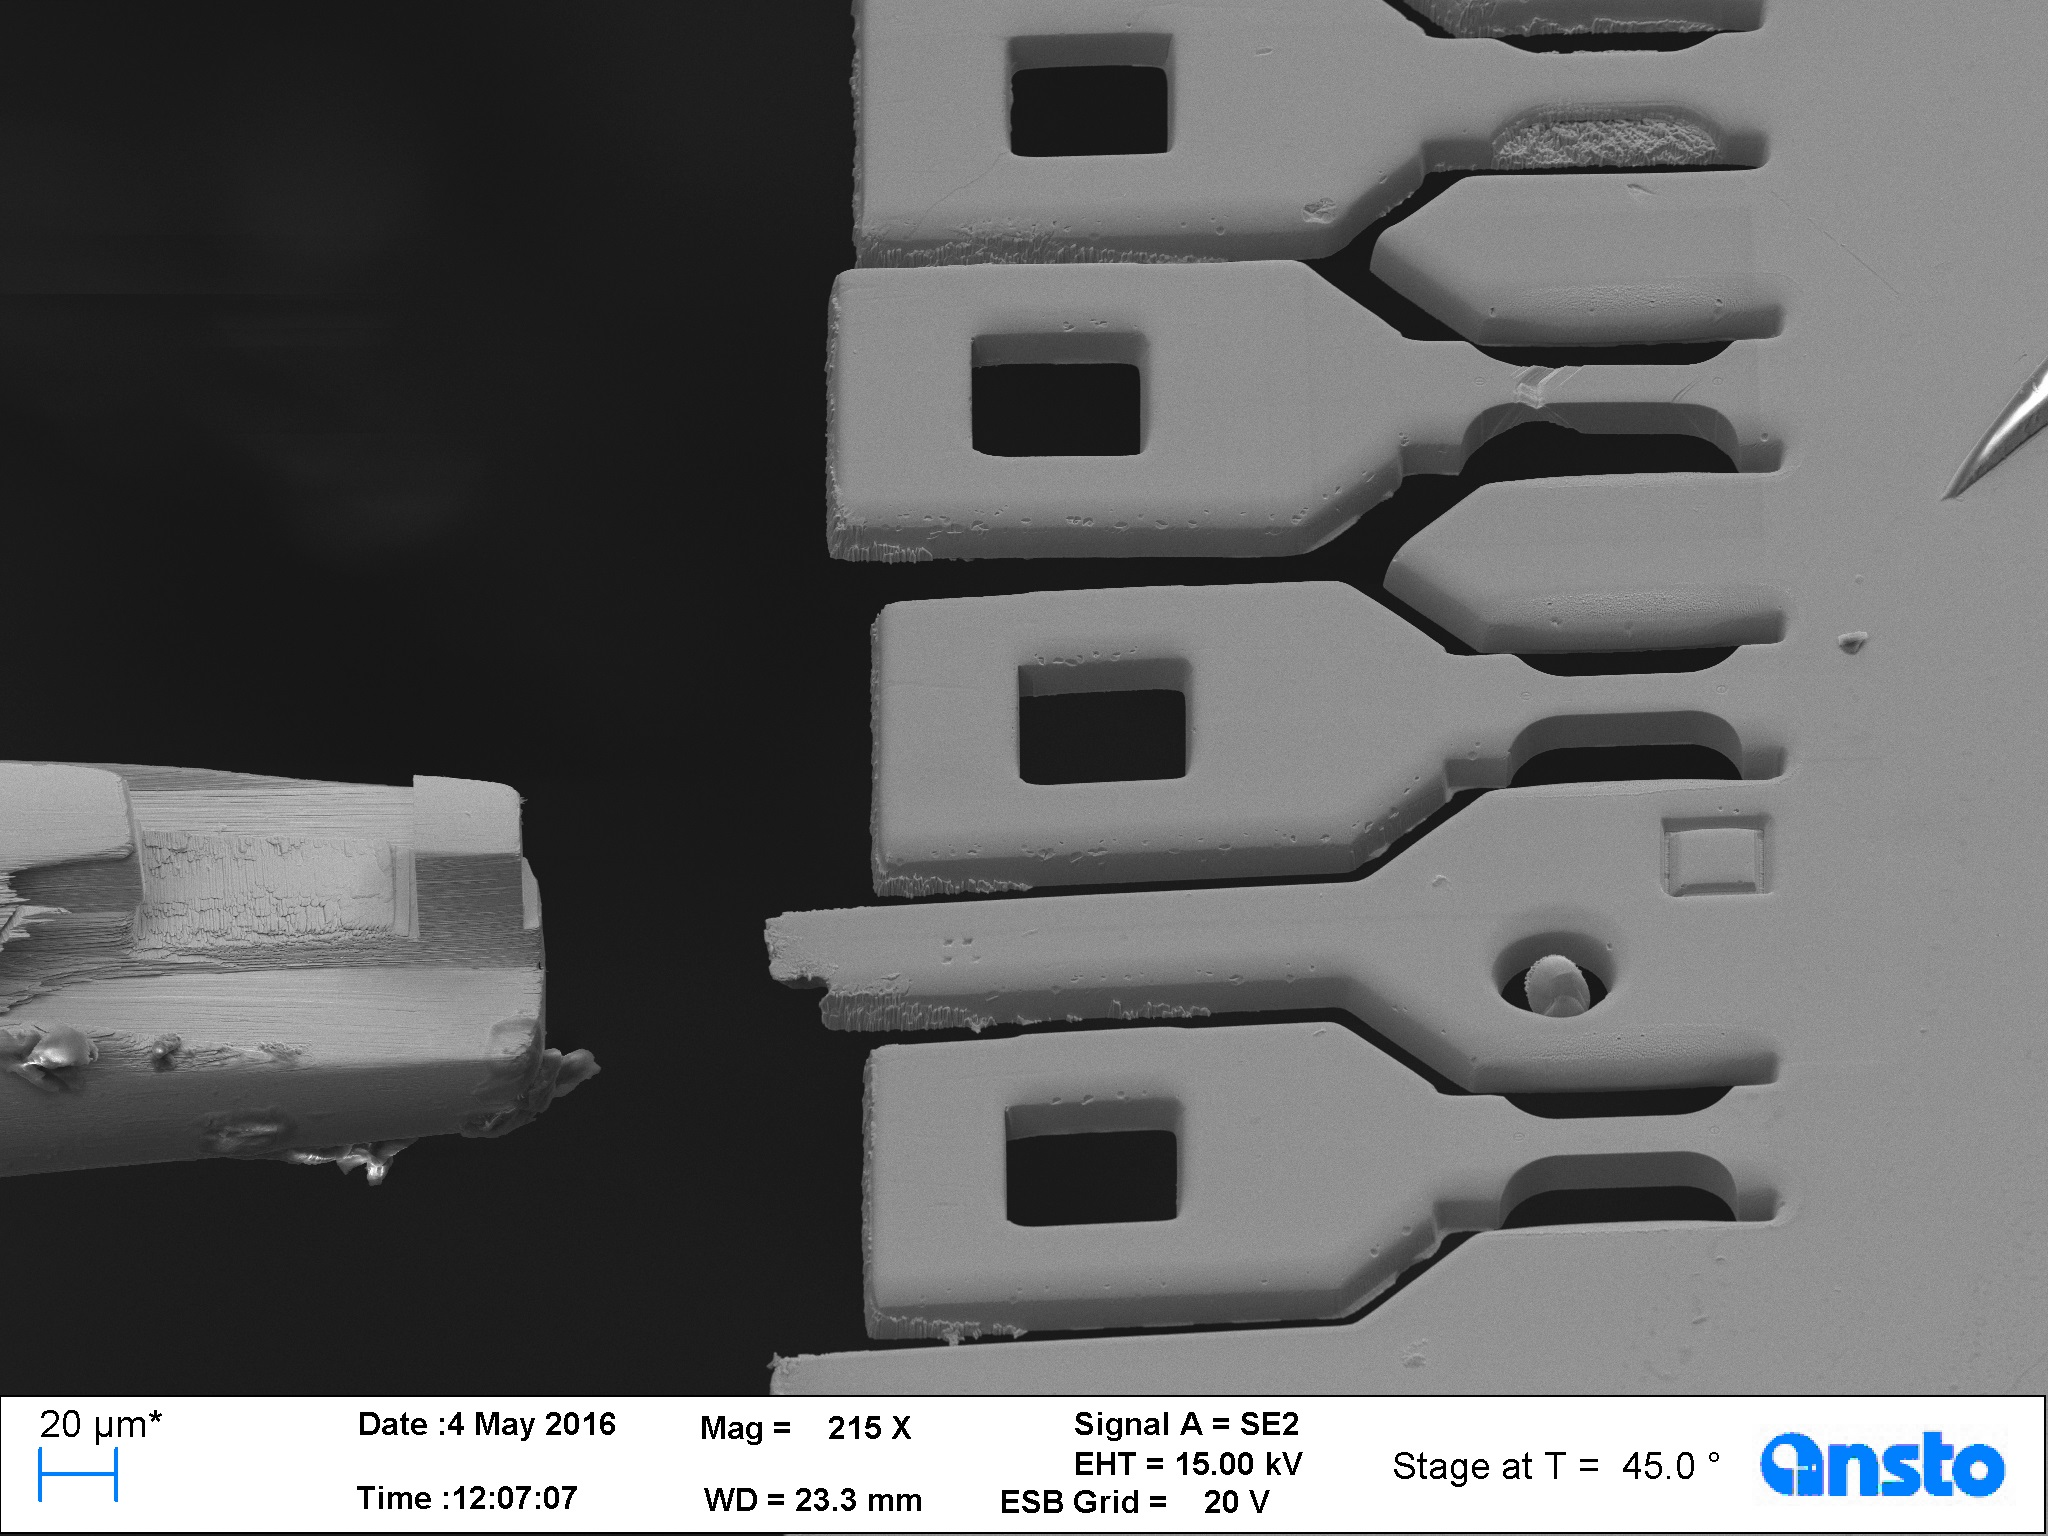
\includegraphics[width=\linewidth]{../data/Ni024.jpg}
        \caption[Stage for micropillar tensile tests.]{Stage for micropillar tensile tests. Ensemble setup, pillars are pulled from the square hole. They are allowed to freely move in the $yz$-plane.}
    \end{subfigure}
    ~
    \begin{subfigure}[t]{0.45\linewidth}
        \centering
        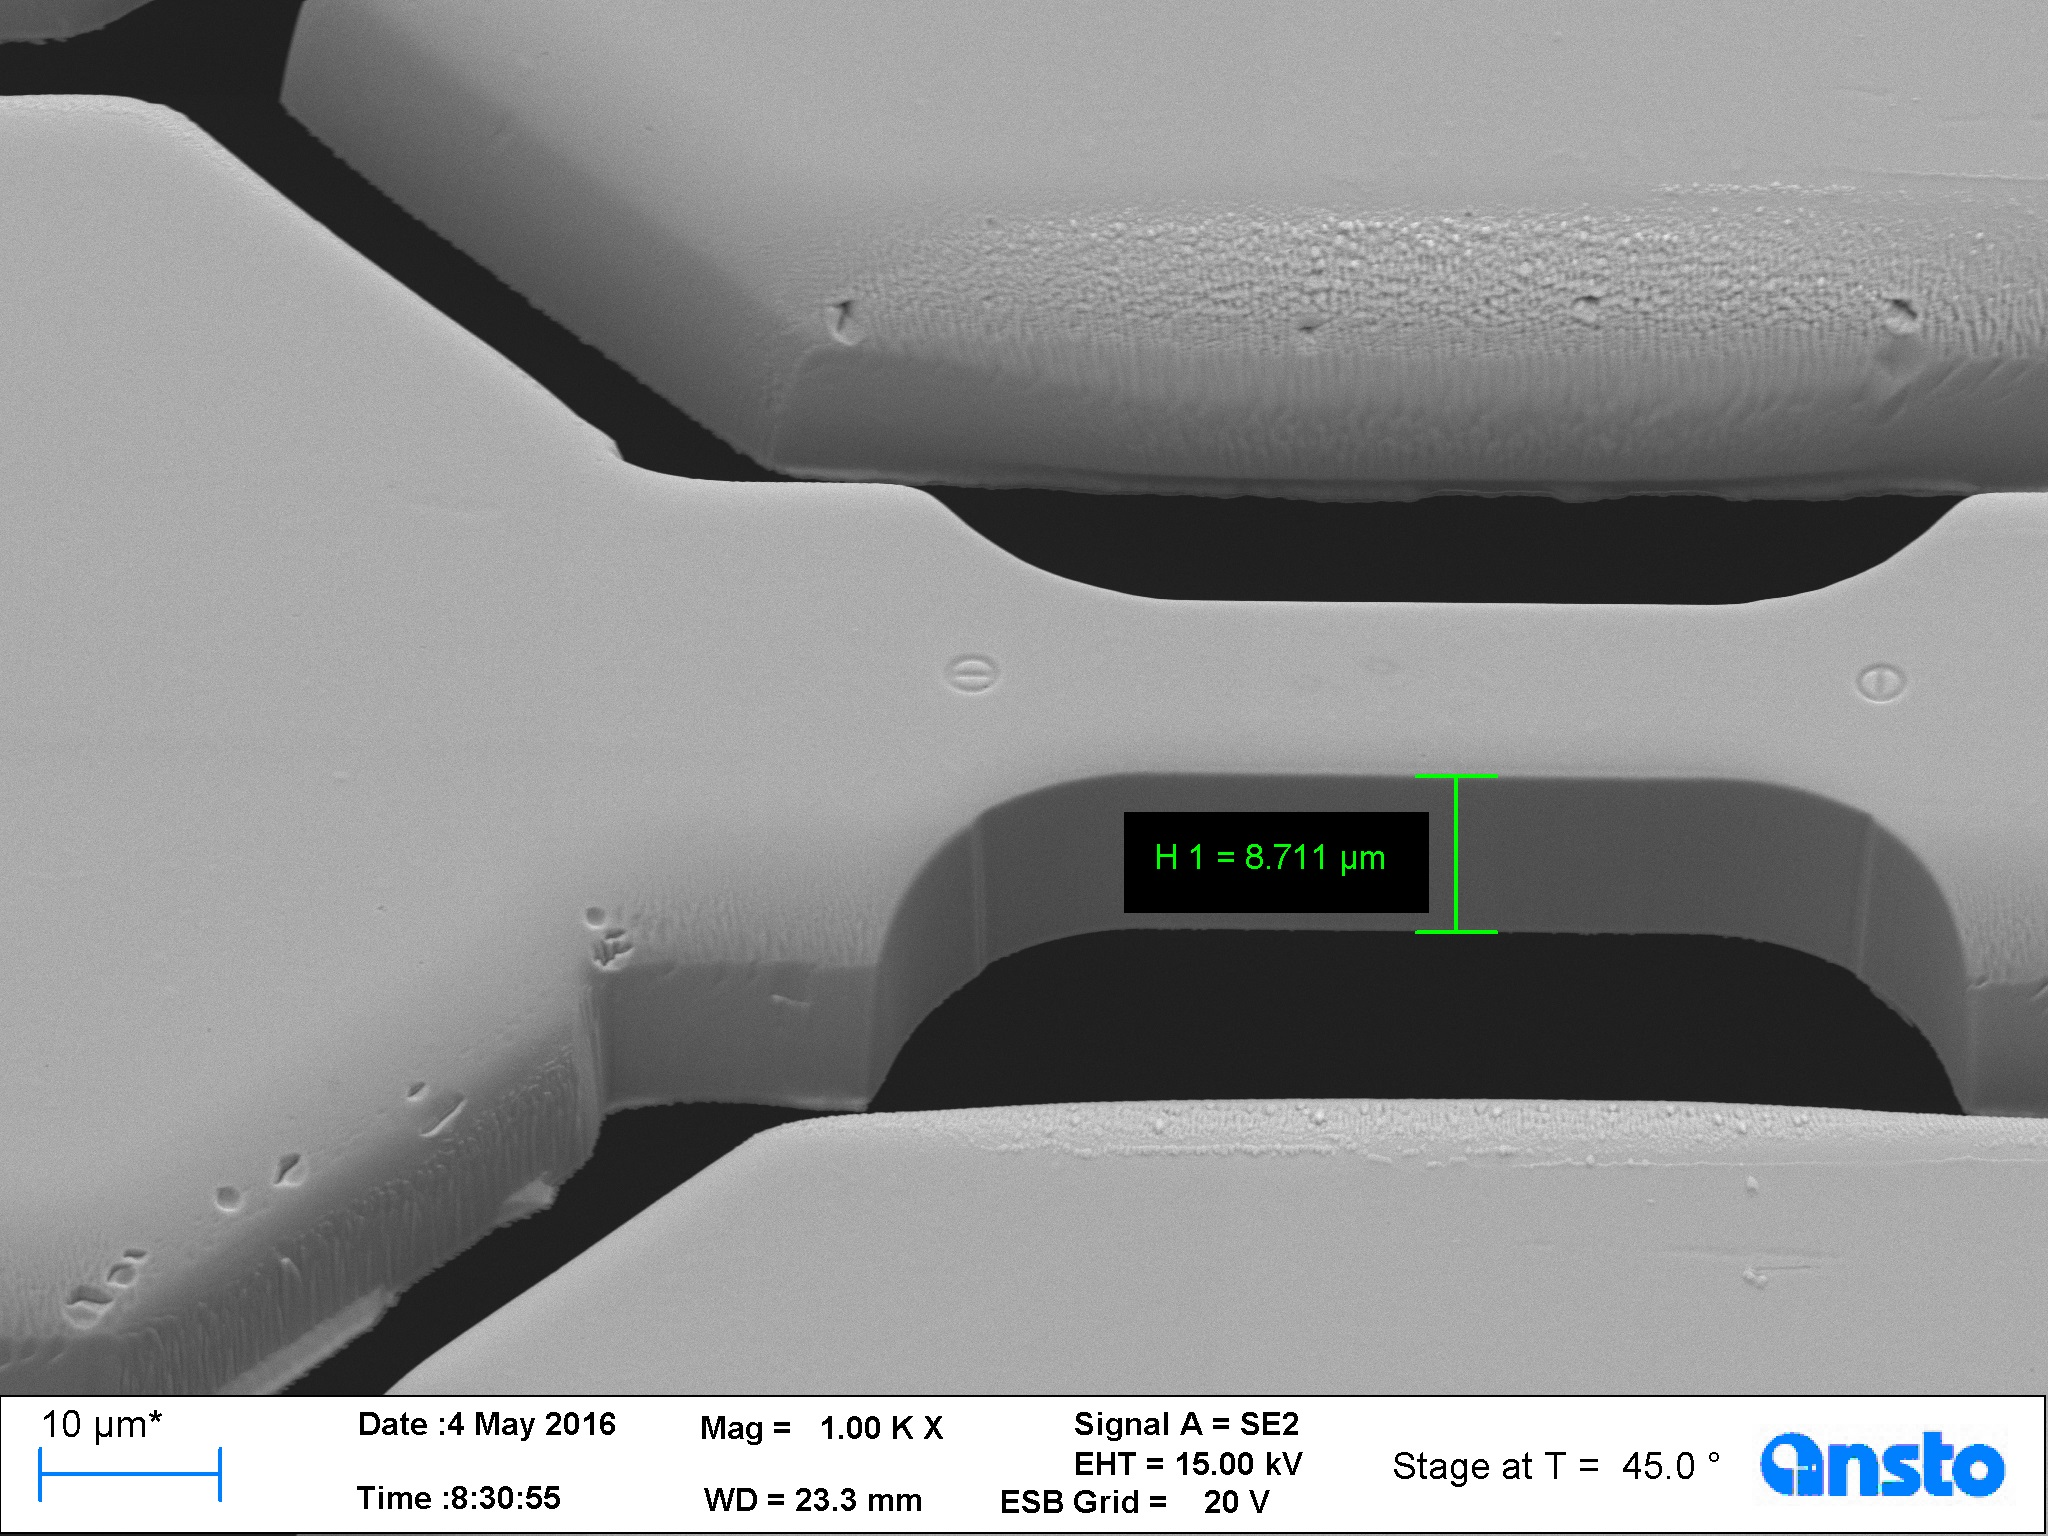
\includegraphics[width=\linewidth]{../data/Ni000.jpg}
        \caption[Close up of the initial state of a single pillar.]{Close up of the initial state of a single pillar. Camera is at $\SI{45}{\degree}$, square cross-section measures $\SI{12}{\micro\metre}$ per side, length is $\sim \SI{30}{\micro\metre}$.}
    \end{subfigure}
    \caption{Experimental stage for tensile tests on Ni micropillars. Provided courtesy of Alan Xu and Dhriti Bhattacharyya from ANSTO Sydney.}
    \label{f:expSetup}
\end{figure}
The load was applied until the pillars failed by necking, as shown in \cref{f:tensileFailure}.
\begin{figure}
    \centering
    \begin{subfigure}[t]{0.3\linewidth}
        \centering
        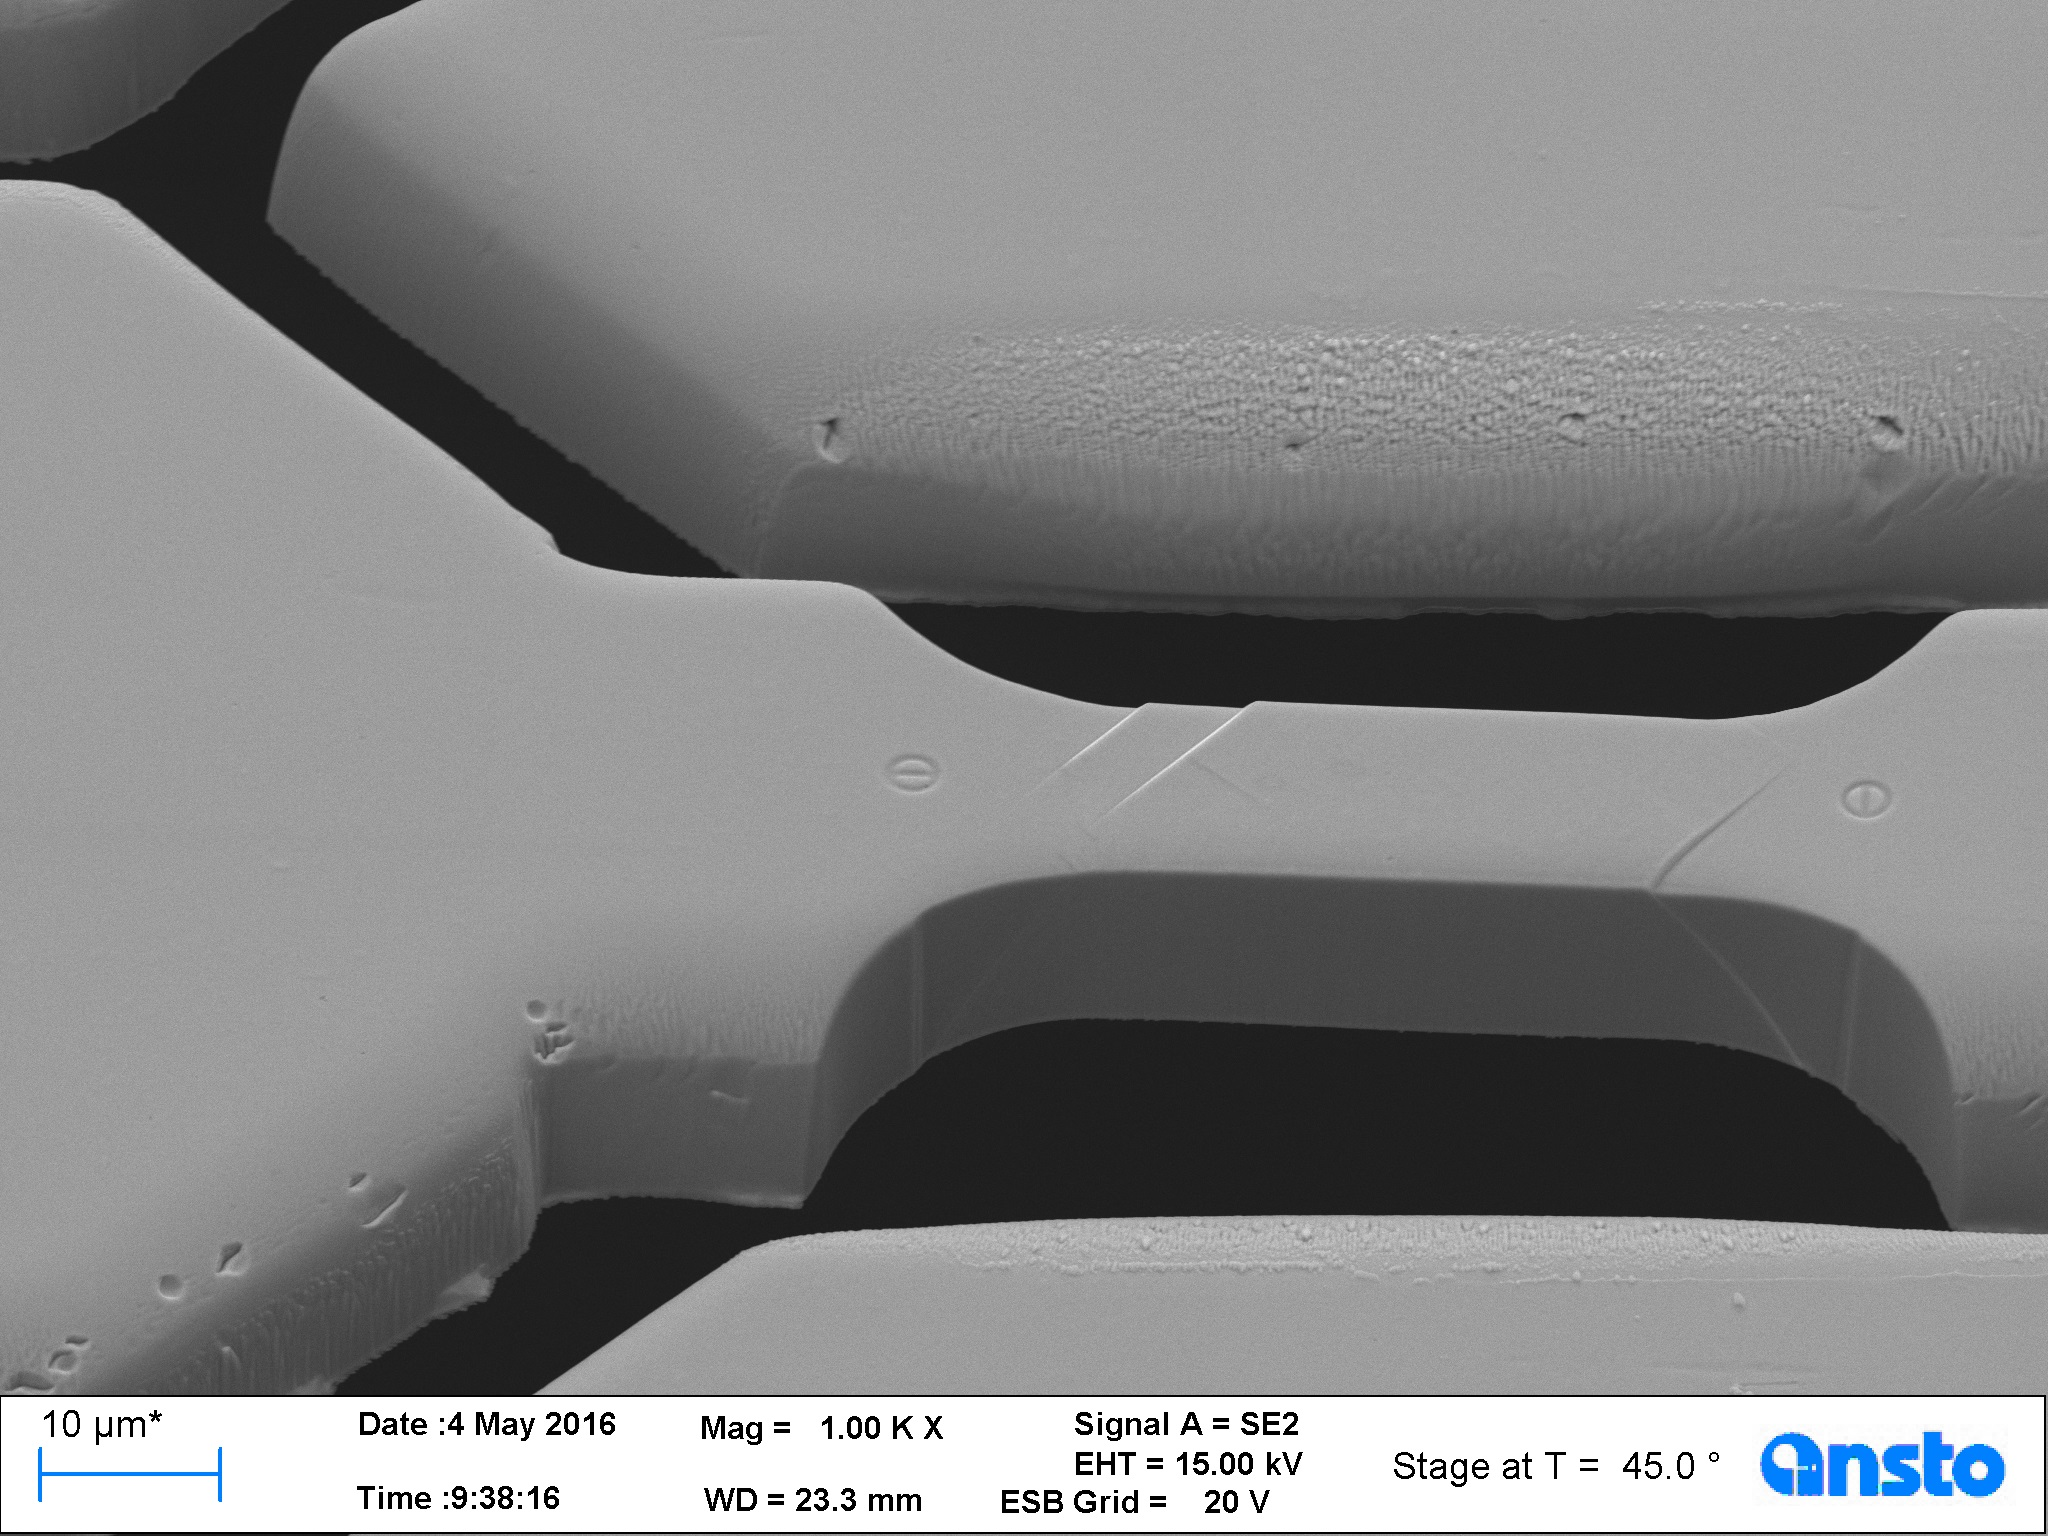
\includegraphics[width=\linewidth]{../data/Ni016.jpg}
    \end{subfigure}
    ~
    \begin{subfigure}[t]{0.3\linewidth}
        \centering
        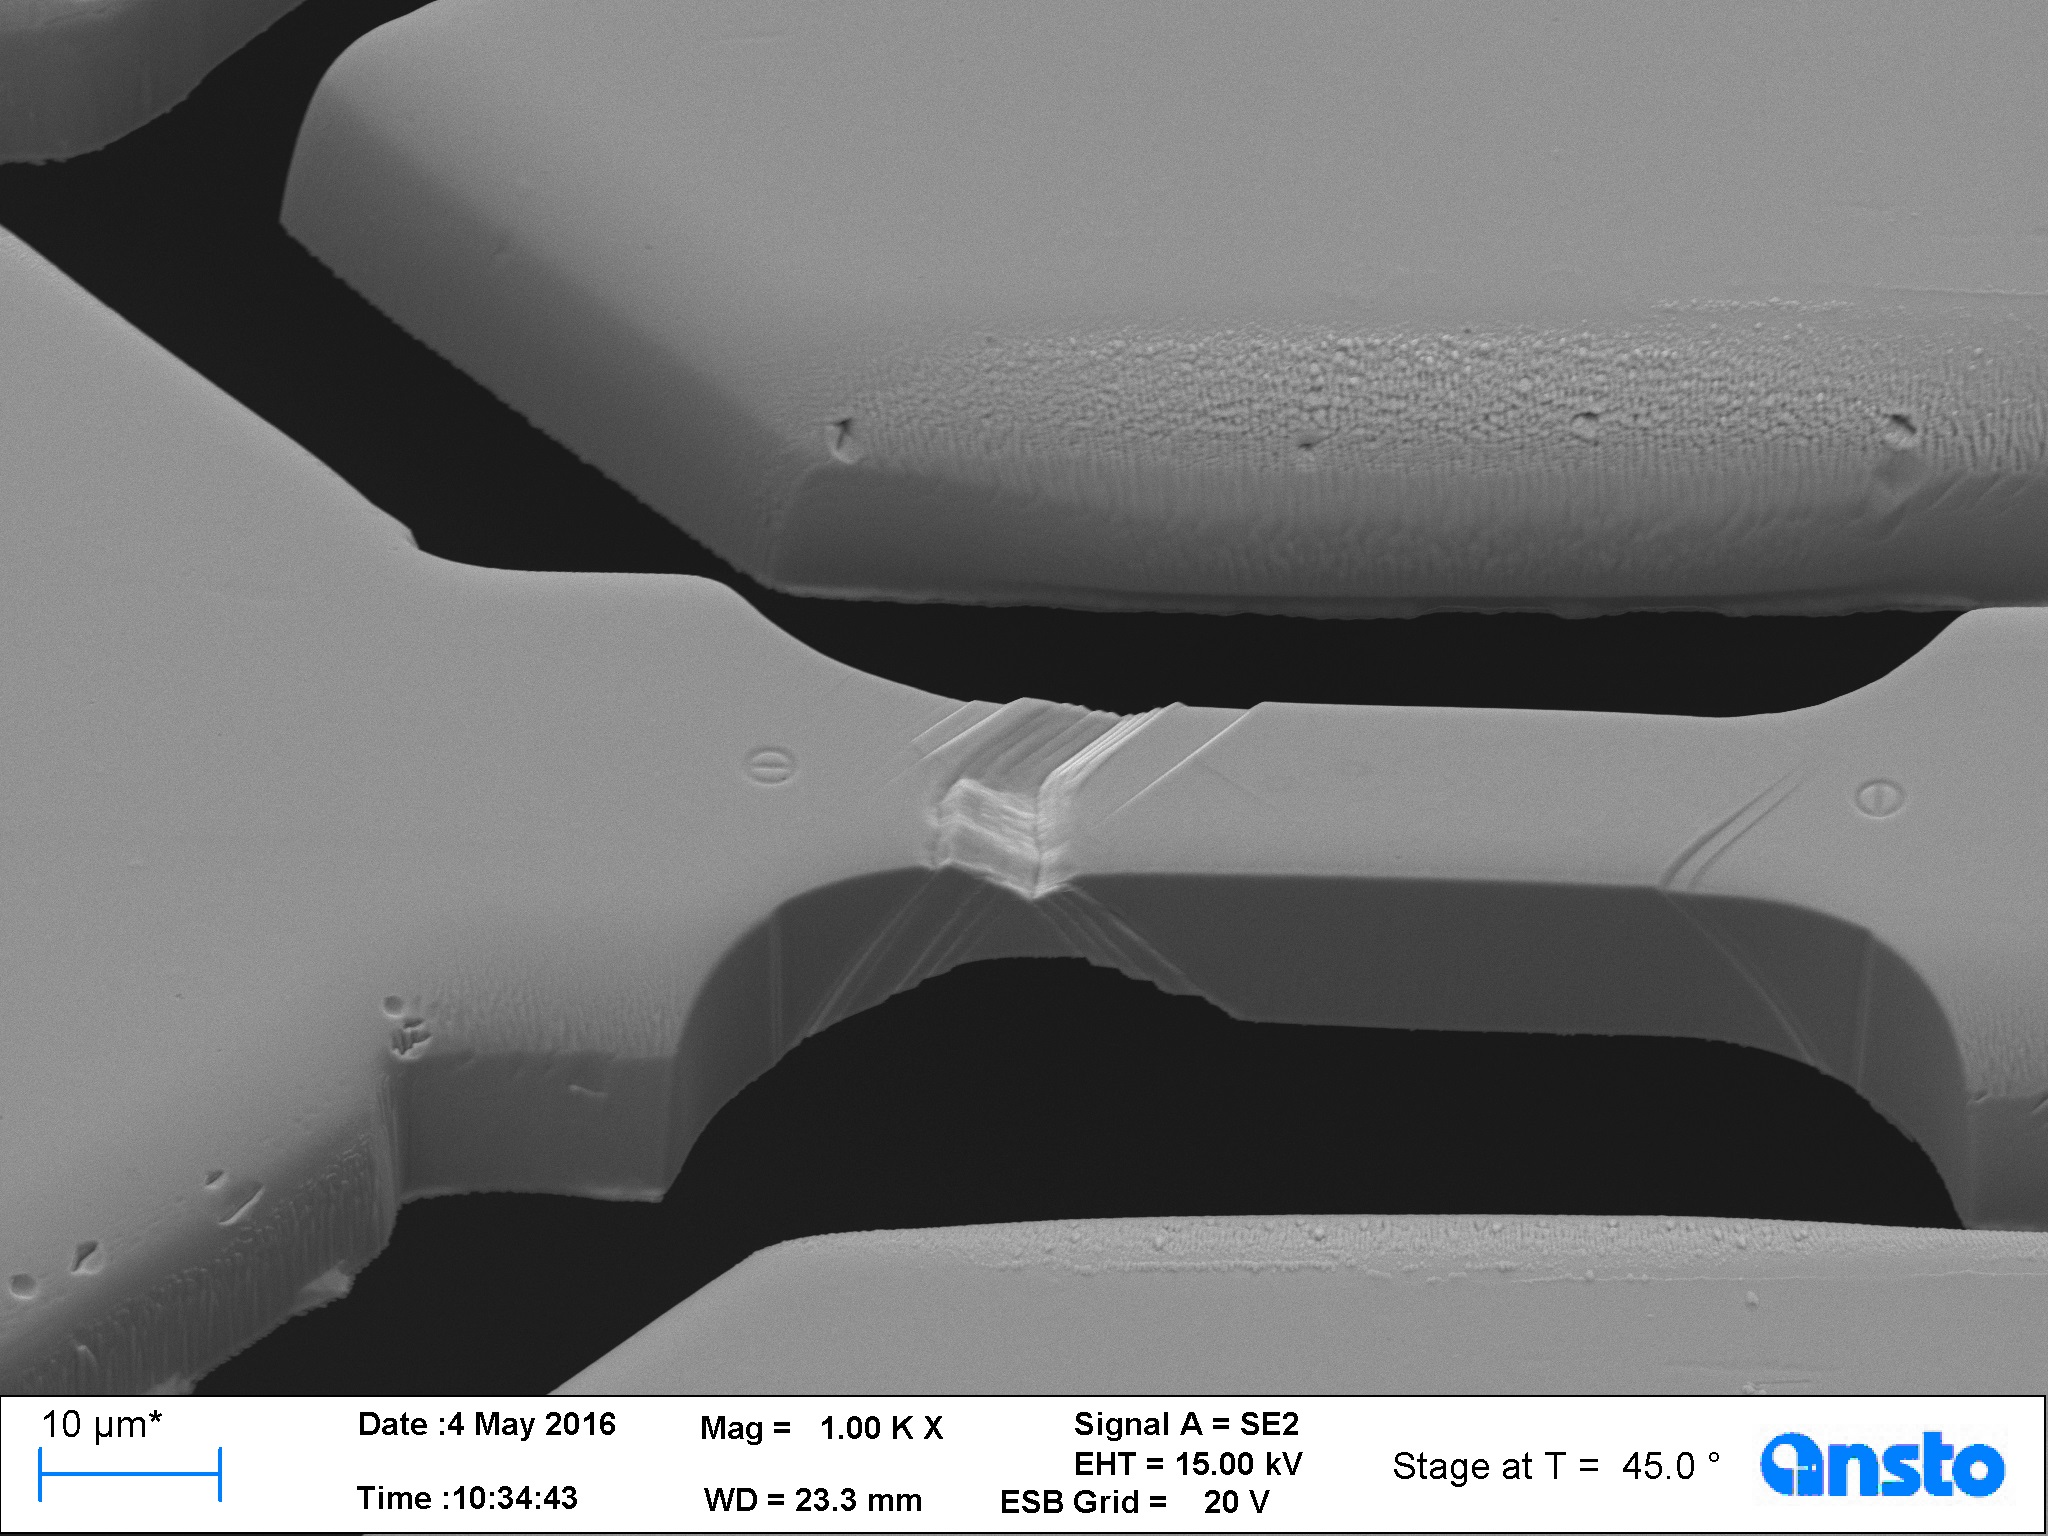
\includegraphics[width=\linewidth]{../data/Ni023.jpg}
    \end{subfigure}
    ~
    \begin{subfigure}[t]{0.3\linewidth}
        \centering
        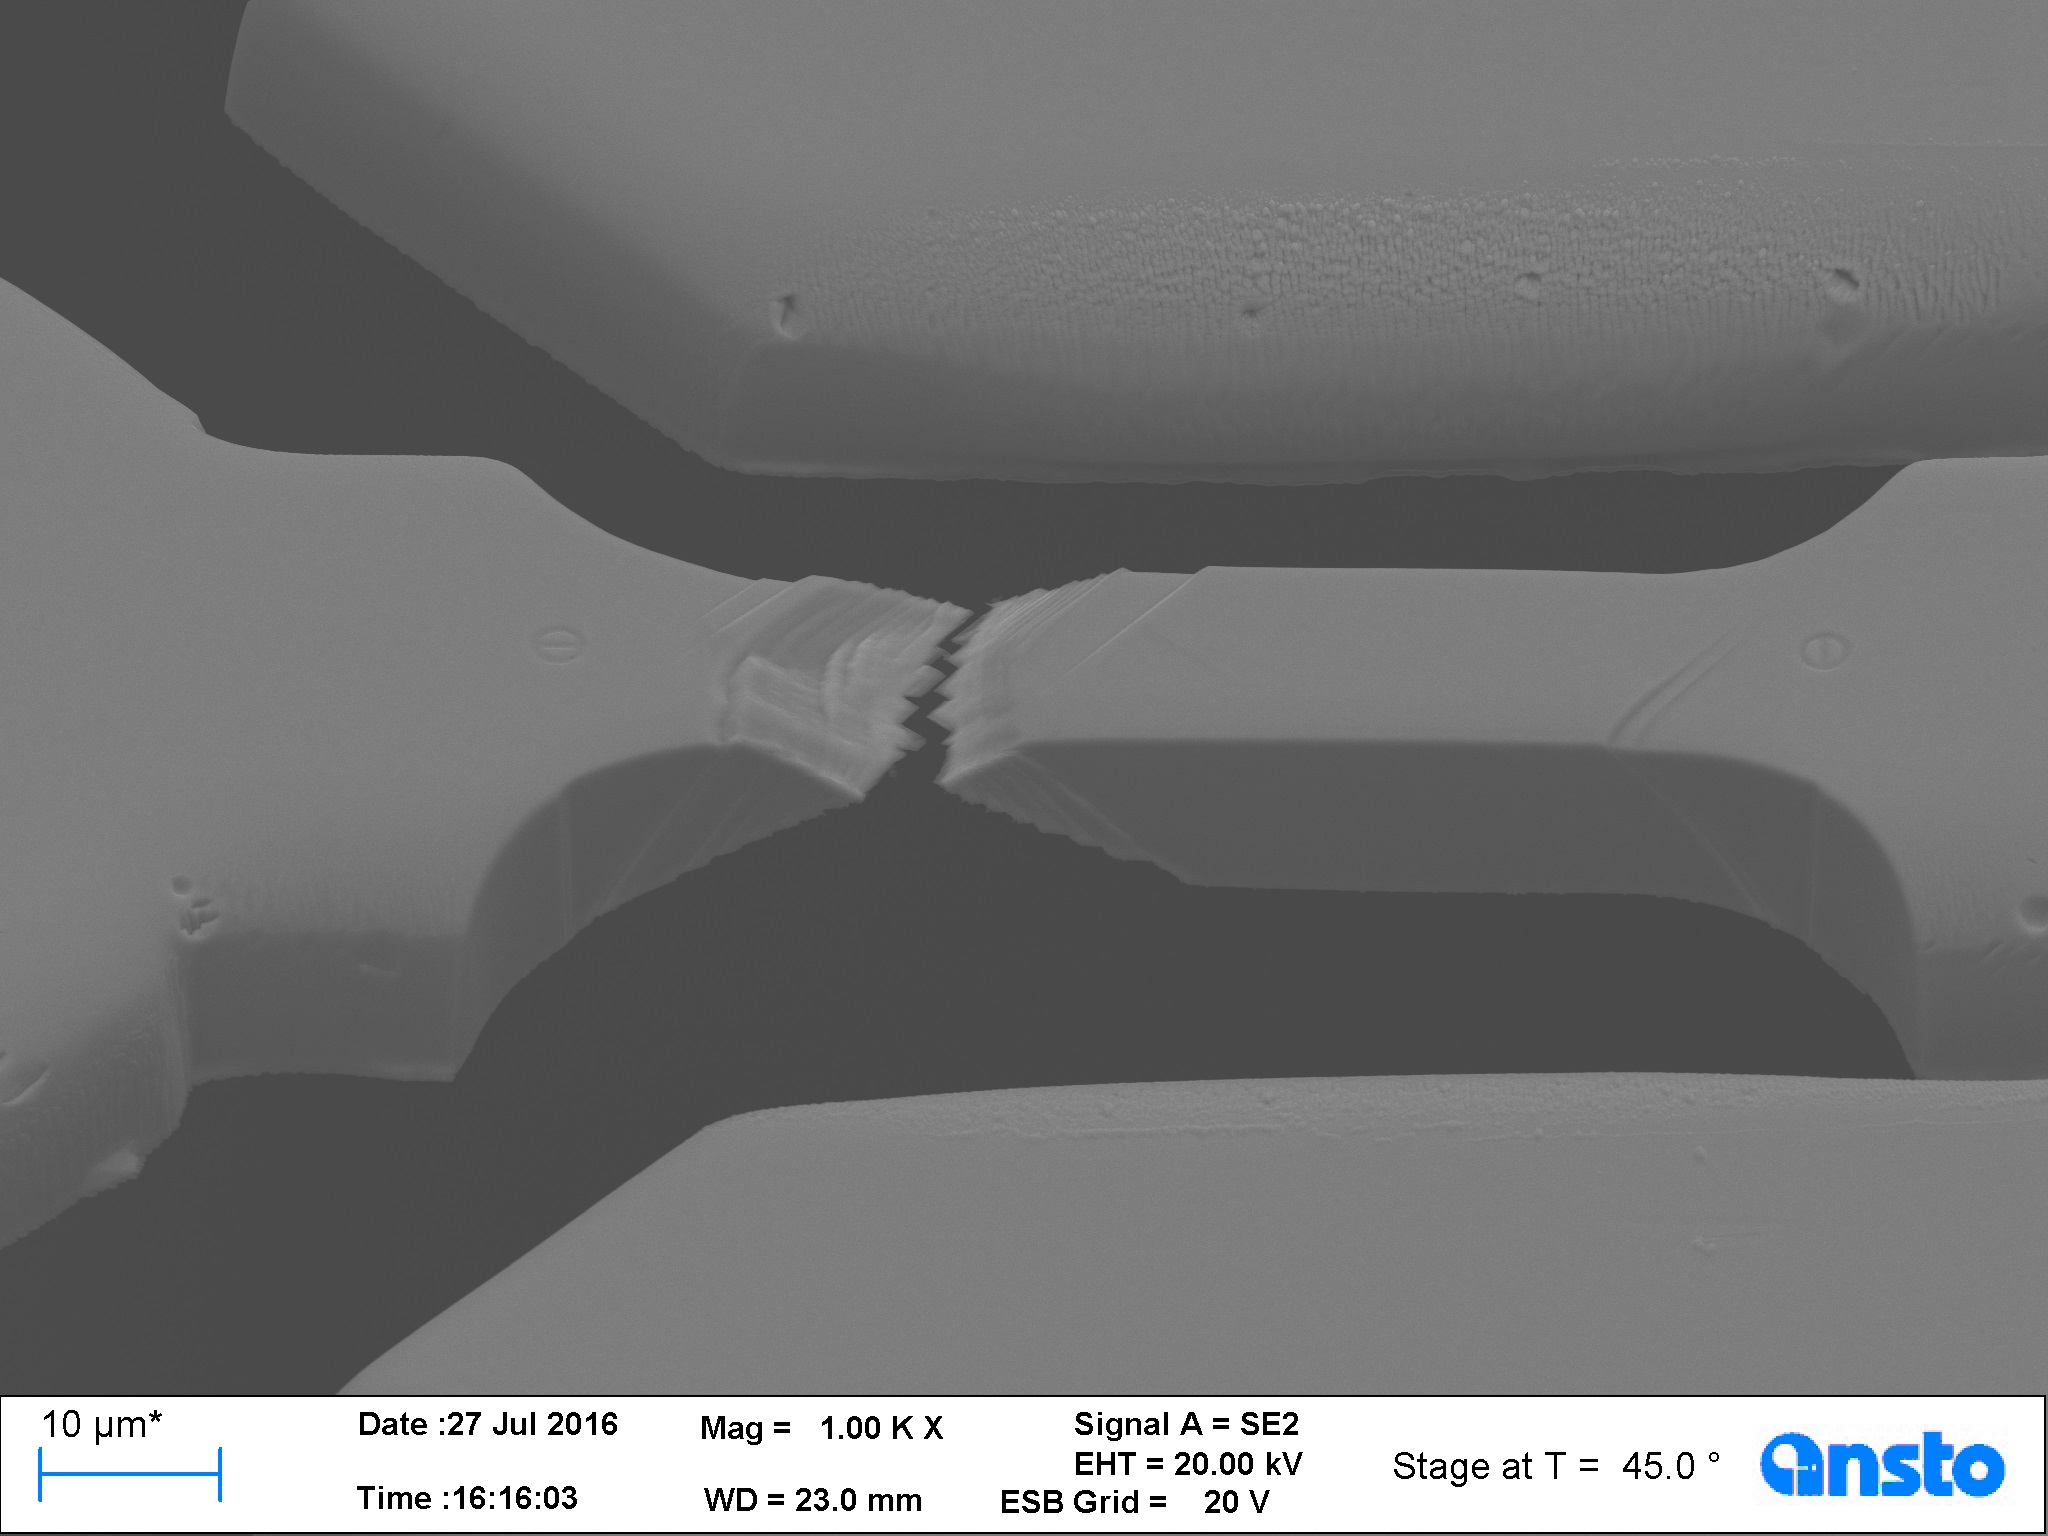
\includegraphics[width=\linewidth]{../data/Ni039.jpg}
    \end{subfigure}
    \caption{Tensile tests taken to failure. Provided courtesy of Alan Xu and Dhriti Bhattacharyya from ANSTO Sydney.}
    \label{f:tensileFailure}
\end{figure}

It is worth noting that the timescale of dislocation plasticity simulations make them unsuitable to simulate the entirety of the experiments. EasyDD does not have a damage law, so it cannot account for fracture. Simulation strain rates are also necessarily higher than experimental ones as discrete dislocation dynamics time scales are on the order of \si{\nano\second}.

\subsection{Dislocation plasticity setup}
\label{ss:modelSetup}

The material parameters of the samples were also not known, so they were estimated from comercially available manufacturing spec sheets and measurements reported from literature. The exact values used for the lattice parameter, shear modulus and Poisson ratio are: $a \coloneqq \SI{3.499}{\angstrom}$, $ \mu  \coloneqq \SI{79}{\giga\pascal}$, $\nu \coloneqq 0.31$ respectively. The lattice parameter is from \cite{ni_lattice} and the othters are the mean of the upper and lower values reported by \cite{azom_nickel}.

We used prismatic loops with four sides as Frank-Read sources to seed the domain with dislocations. Each side of the square sources had two segments of equal length (8 segments per source). Because we used Frank-Read sources, only two opposite sides per source were allowed to move, the others were pinned.

Preliminary simulations showed the initially assumed dislocation density necessitated the initial sources be quite small, so the yield stress of the simulation was much greater than what was experimentally observed. We therefore dropped the number of sources to a single seed loop per active slip system, while increasing the size of each source. For the $\langle 1\, 0\, 0 \rangle$ loading direction, this was 8 loops, and for $\langle 1\, 1\, 0 \rangle$ it was only 4; \cref{t:slipSystems} contains the active slip systems for both scenarios.
\begin{table}
    \centering
    \caption{Active FCC slip systems for prismatic loops in the $\langle 1\, 0\, 0 \rangle$ and $\langle 1\, 1\, 0 \rangle$ tensile loading directions.}
    \label{t:slipSystems}
    \begin{tabular}{rcl}
        \toprule
        Loading direction                            & Slip plane                          & Burgers vector                      \\
        \midrule
        \multirow{8}{*}{$\langle 1\, 0\, 0 \rangle$} & $\left(1\, 1\, 1\right)$            & $\left[1\, \overline{1}\, 0\right]$ \\
                                                     & $\left(1\, 1\, 1\right)$            & $\left[1\, 0\, \overline{1}\right]$ \\
                                                     & $\left(\overline{1}\, 1\, 1\right)$ & $\left[1\, 1\, 0\right]$            \\
                                                     & $\left(\overline{1}\, 1\, 1\right)$ & $\left[1\, 0\, 1\right]$            \\
                                                     & $\left(1\, \overline{1}\, 1\right)$ & $\left[1\, 1\, 0\right]$            \\
                                                     & $\left(1\, \overline{1}\, 1\right)$ & $\left[1\, 0\, \overline{1}\right]$ \\
                                                     & $\left(1\, 1\, \overline{1}\right)$ & $\left[1\, 0\, 1\right]$            \\
                                                     & $\left(1\, 1\, \overline{1}\right)$ & $\left[1\, \overline{1}\, 0\right]$ \\
        \midrule
        \multirow{4}{*}{$\langle 1\, 1\, 0 \rangle$} & $\left(\overline{1}   1   1\right)$ & $\left[1\, 0\, 1\right]$            \\
                                                     & $\left(\overline{1}   1   1\right)$ & $\left[0\, 1\, \overline{1}\right]$ \\
                                                     & $\left(1  \overline{1}   1\right)$  & $\left[0\, 1\, 1\right]$            \\
                                                     & $\left(1  \overline{1}   1\right)$  & $\left[1\, 0\, \overline{1}\right]$ \\
        \bottomrule
    \end{tabular}
\end{table}
To minimise computation expenditure, we only included these active slip systems in our simulations. This obviously does not fully represent reality, but it saves simulations from having to resolve as many collisions and topological operations as would otherwise occur. Regardless of this decision, the simulations still managed to do an unexpectedly great job at quantitatively, and qualitatively reproducing the experimentally measured strain-stress curves as discussed in \cref{s:NiResults}.

The pillar length was defined as $\SI{42}{\micro\metre}$, or $3.5\times$ the length of one of the $\SI{12}{\micro\metre}$ sides of the square cross-section. The extra length acts as a buffer zone for simulating dislocations moving into the bulk, where they pile up. In the simulation, they get pinned to the end of the cantilever as per \cref{s:surfRem}. The initial FR sources were random-uniformly distributed within the central $80\%$ of the domain, i.e. $x \in [0.1X, 0.9X]$, where $x$ is a point along dimension $X$. Given the fact that the number of sources was quite low, various distributions were generated until we arrived at one that spanned the whole domain, rather than clustered about a region.

We define surface node sets $\left\{\forall (x, y, z) \in [0,\, 1] \vert S_{xyz} \in \partial \hat{V}\right\}$, where $\hat{V}$ is a unit volume such that $S_{000}$ denotes the node at the origin, $S_{x00}$ the $x$-axis spanning edge at $y,\, z=0$, and $S_{xy0}$ the $xy$-plane at $z=0$. We use these node sets to define our Neuman (displacement) boundary conditions as follows,
\begin{subequations}
    \begin{align}
        u_x(0, y, z) & = 0    \\
        u_y(0, Y, z) & = 0    \\
        u_z(0, y, 0) & = 0    \\
        u_x(X, y, z) & = U\,. \\
        % S_{0yz},\, S_{0y0},\, S_{0y1},\, S_{00z},\, S_{01z},\, S_{000},\, S_{001},\, S_{010},\, S_{011} & \gets u_x = 0        \\
        % S_{01z},\, S_{010},\, S_{011}                                                                   & \gets u_y = 0        \\
        % S_{0y0},\, S_{010},\, S_{000}                                                                   & \gets u_z = 0        \\
        % S_{1yz},\, S_{1y0},\, S_{1y1},\, S_{10z},\, S_{11z},\, S_{100},\, S_{101},\, S_{110},\, S_{111} & \gets u_x = U > 0\,.
    \end{align}
\end{subequations}
Where $X$ and $Y$ are the upper limits of the FE domain in the $x$ and $y$-direction. Once mapped to our simulated cuboid geometry, it looks like \cref{f:tensileSetup}. All other degrees of freedom are free to move.
\begin{figure}
    \centering
    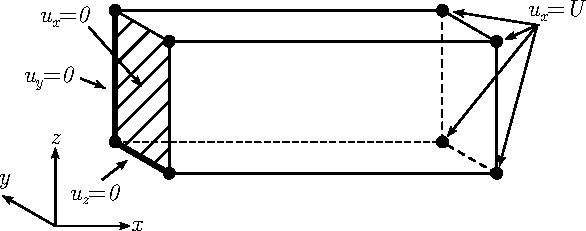
\includegraphics[width=0.8\linewidth]{tensileSetup.pdf}
    \caption[Displacement boundary conditions for dislocation plasticity modelling of single crystal, micro-tensile tests.]{Displacement boundary conditions for dislocation plasticity modelling of single crystal, micro-tensile tests.}
    \label{f:tensileSetup}
\end{figure}

In EasyDD, time is defined in units of shear modulus \cref{eq:timeConversion},
\begin{align}\label{eq:timeConversion}
    t_{\rvar{real}} & = t_{\rvar{sim}} \dfrac{B}{\mu}\,.
\end{align}
In EasyDD the dislocation mobility, $B \coloneqq 1$ and $\mu \coloneqq 1$. However, $B$ has units of $\si{\pascal\,\second\,b^{\overline{1}}}$, and $\mu$ units of $\si{\pascal}$. In order to estimate our strain rate, we used a generic value for an FCC transition metal of $B = \SI{1e-4}{\pascal\,\second}$, and used similar heuristics as described in \cite[p.~237]{ddlab}.

The experimental strain rates were $\SI{5}{\nano\metre\per\second}$ and $\SI{500}{\nano\metre\per\second}$, give simulation strain rates that are far too low for the timescales we can simulate. However, as mentioned in \cref{ss:matrix}, it is important that a quasistatic condition is met for the mobility functions to hold. We therefore chose a strain rate that enabled simulations to advance sufficiently, without overloading the system. We settled on multiplying the converted value\footnote{The converted value used in the simulations is $\left(\SI{5e-3}{\micro\metre}/a\right) \times \left(B /  \mu \right)$, where $a$ is the lattice parameter in micrometers, $B$ the dislocation mobility and $ \mu $ the magnitude of the shear modulus from \cref{eq:timeConversion}.} of the $\SI{5}{\nano\metre\per\second}$ strain rate by a factor of $5 \times 10^6$, which corresponds to a strain rate of $\SI{2.5}{\centi\metre\per\second}$. Any higher and the yield point increased, any lower and the simulations took much longer to advance without a significant change in the dislocation structure and strain-stress curve.

Two different initial source segment lengths, $L$, were trialed for each loading direction. As previously mentined, each square source was made up of 8 equal segments. Source sizes were calculated based on estimates of the yield stress, $\sigma_\rvar{y}$, suggested by Alan and Dhriti, but had to be adjusted for the simulation's higher strain rate. We did not directly use \cref{eq:yieldStress}, but $l = 2 \mu b / \sigma_\rvar{y}$, to account for the sources being at an angle with respect to the loading direction\footnote{Perhaps it would be more accurate to drop the factor of two and use the critically resolved shear stress instead of the yield stress directly, $\tau = \cos(\phi)\cos(\lambda) \sigma_\rvar{y}$, where $\phi$ and $\lambda$ are the angles between the applied stress, glide plane normal, and glide direction respectively. However, a number of much stronger assumptions and adjustments had already been made, and this worked satisfactorily.}. This gave two source size parameters for each direction. This data is summarised in \cref{t:sourceSize}.
\begin{table}
    \centering
    \caption{Source parameters used for the simulations. Loading direction; estimated experimental yield stress, $\sigma_\rvar{y}$ in \si{\mega\pascal}; source segment length, $L$ in \si{\micro\metre}; and initial dislocation density, $\rho$ in dislocations \si{\micro\metre^{-2}}.}
    \label{t:sourceSize}
    \begin{tabular}{rccl}
        \toprule
        Loading direction                            & $\sigma_\rvar{y}$ & $L$    & $\rho$              \\
        \midrule
        \multirow{2}{*}{$\langle 1\, 0\, 0 \rangle$} & 183               & 0.8545 & $4.5\times 10^{-3}$ \\
                                                     & 142               & 1.1012 & $5.8\times 10^{-3}$ \\
        \midrule
        \multirow{2}{*}{$\langle 1\, 1\, 0 \rangle$} & 158               & 0.9897 & $2.6\times 10^{-3}$ \\
                                                     & 101               & 1.5482 & $4.1\times 10^{-3}$ \\
        \bottomrule
    \end{tabular}
\end{table}

All simulations ran for approximately 5 weeks. They did not use the new power dissipation strategy for collision-separation because that development came a few weeks after the simulations started running, and other computational resources were of critical importance to other users.

\section{Results and discussion}
\label{s:NiResults}

The experimental measurements go up to fracture, well beyond the domain of dislocation plasticity simulations; they also discard the elastic region, and the early onset of plasticity as shown in \cref{sf:Ni100,sf:Ni110}. Conversely, dislocation plasticity simulations are limited to small strains, i.e. the part of the curves that typically fall below the experimental limit of detection as shown in \cref{sf:Ni100_DDD,sf:Ni110_DDD}. However, they can elucidate dislocation mechanisms behind plasticity. Here, dislocation plasticity serves as a bridge between the elastic and plastic regimes and lets us explore the mechanisms behind the differences in strain-stress curves between the $\langle 1\,0\,0 \rangle$ and $\langle 1\,1\,0 \rangle$ loading directions.

\begin{figure}
    \centering
    \begin{subfigure}[t]{0.45\linewidth}
        \centering
        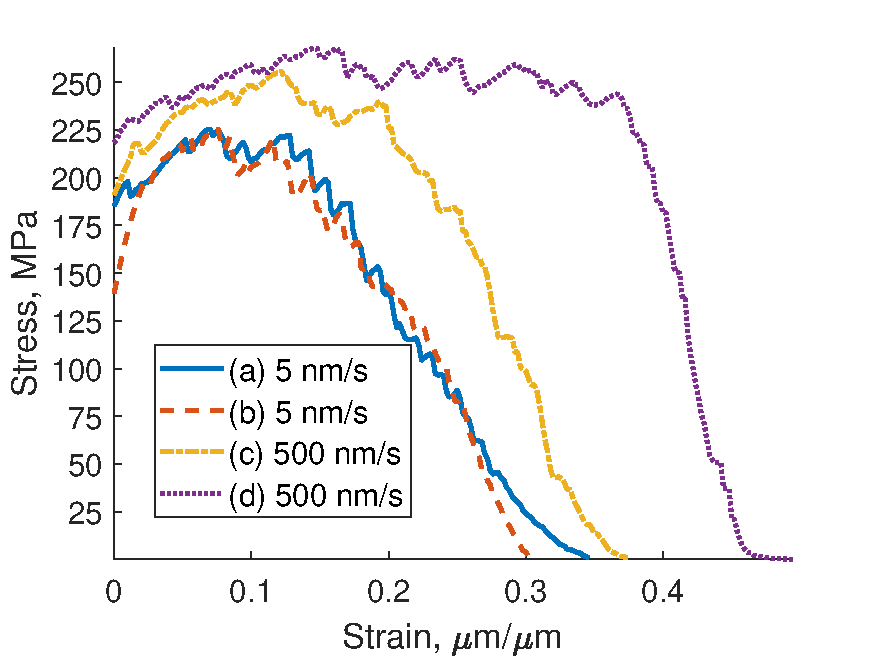
\includegraphics[width=\linewidth]{../data/Ni100.pdf}
        \caption{Experimental results of tensile loading of a Ni monocrystal in $\langle 1\, 0\, 0 \rangle$.}
        \label{sf:Ni100}
    \end{subfigure}
    ~
    \begin{subfigure}[t]{0.45\linewidth}
        \centering
        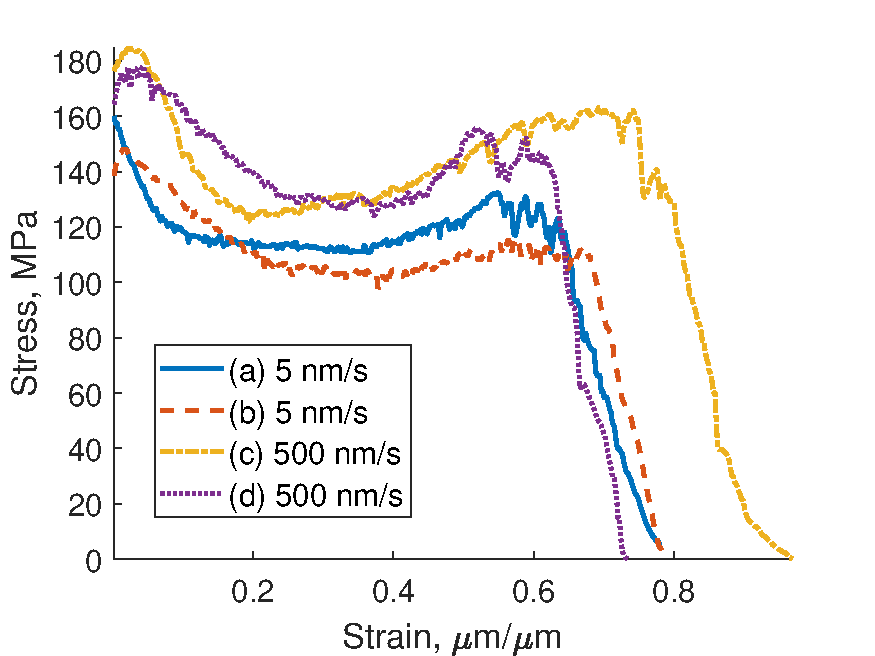
\includegraphics[width=\linewidth]{../data/Ni110.pdf}
        \caption{Experimental results of tensile loading of a Ni monocrystal in  $\langle 1\, 1\, 0 \rangle$.}
        \label{sf:Ni110}
    \end{subfigure}

    \begin{subfigure}[t]{0.45\linewidth}
        \centering
        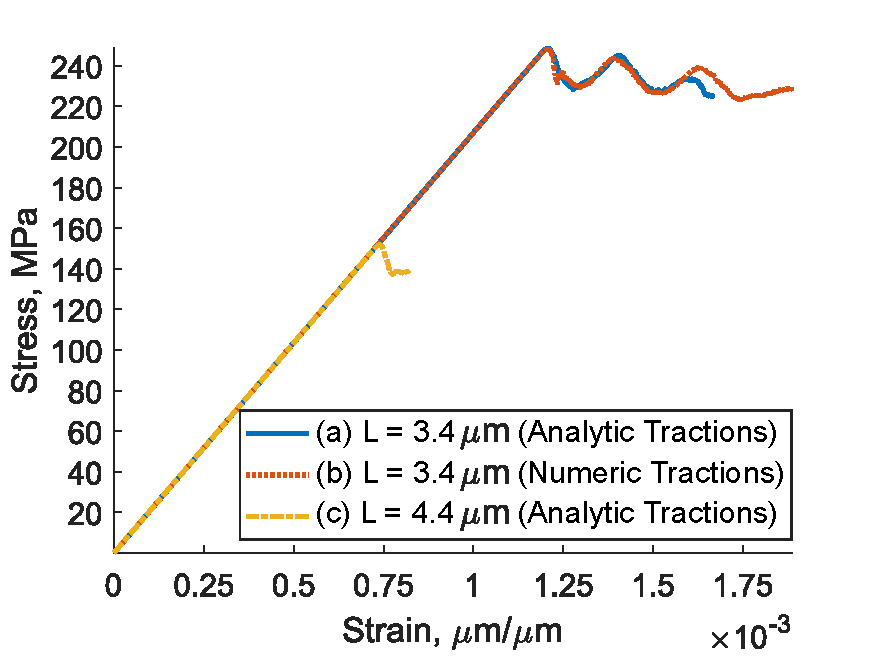
\includegraphics[width=\linewidth]{../data/Ni100_DDD.pdf}
        \caption[Dislocation-Plasticity simulation of tensile loading of Ni in $\langle 1\, 0\, 0 \rangle$.]{Dislocation-Plasticity simulation of tensile loading of Ni in $\langle 1\, 0\, 0 \rangle$.}
        \label{sf:Ni100_DDD}
    \end{subfigure}
    ~
    \begin{subfigure}[t]{0.45\linewidth}
        \centering
        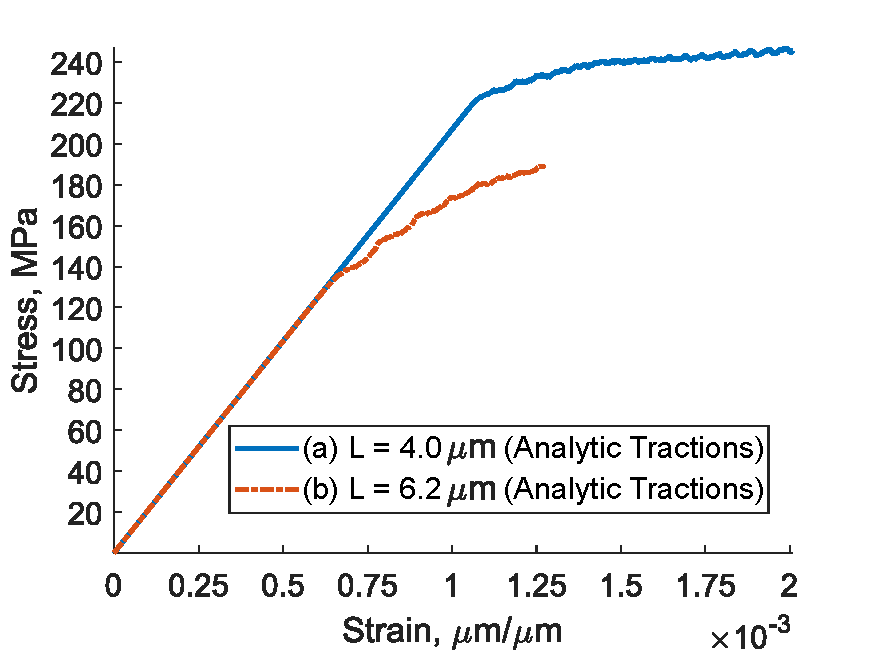
\includegraphics[width=\linewidth]{../data/Ni110_DDD.pdf}
        \caption[Dislocation-Plasticity simulation of tensile loading of Ni in $\langle 1\, 1\, 0 \rangle$.]{Dislocation-Plasticity simulation of tensile loading of Ni  in $\langle 1\, 1\, 0 \rangle$.}
        \label{sf:Ni110_DDD}
    \end{subfigure}
    \caption{Experimental and simulated strain-stress curves of Ni micropillar tensile tests. The simulations used different source sizes, $L$ but kept the strain rate the same at $\SI{2.5}{\centi\metre\per\second}$}
    \label{f:NiStrainStress}
\end{figure}

\Cref{sf:Ni100,sf:Ni110} show the experimental strain-stress curves for the $\langle 1\,0\,0 \rangle$ and $\langle 1\,1\,0 \rangle$, respecively. As expected, higher strain rates mean higher stresses overall, and different loading directions produce very different graphs. However, there is quite a large variation between samples even within similar strain rates. This points at dislocations having quite a large effect on the outcome of the experiment. The difference in shape between graphs of both loading directions also points to different slip systems activating at different strains and behaving quite differently from each other.

The experimentally obtained strain-stress curve for the $\langle 1\,0\,0 \rangle$ loading direction (\cref{sf:Ni100}) show fairly distinguishable features. The curves for the $\SI{5}{\nano\meter\per\second}$ strain rate, (a) and (b), are both quite similar for most of their domain. However, one of the samples yields close to $\SI{140}{\mega\pascal}$ and fails at $30\%$ strain, while the other yields at around $\SI{180}{\mega\pascal}$ and fails closer to $35\%$. These are not insignificant differences, especially at small scales. However, the bulk of the curves look quite similar to one another, and very different to the higher strain rate curves. Those for the $\SI{500}{\nano\metre\per\second}$ strain rate, (c) and (d), are quite different from each another. Of note is the yield point of (c), which is at approximately the same point as (a) despite having $100\times$ larger strain rate. Moreover, the difference between the failure points of (c) and (a) is less than the difference between (a) and (b) despite the difference in strain rate, and very different from the failure point of the other high strain rate cuve, (d). That said, both high strain rate curves, (c) and (d), are subjected to higher overall stresses and fail at higher strains than lower strain rate curves, (a) and (b). These observations appear to indicate that strain rates at this scale may be important to dislocation behaviour in this loading direction. Unfortunately, more sound conclusions cannot be drawn without more samples at different strain rates.

The experimentally obtained strain-stress curves in the $\langle 1\,1\,0\rangle$ loading direction are much more homogenous (\cref{sf:Ni110}). The curves corresponding to $\SI{5}{\nano\metre\per\second}$ strain rates, (a) and (b), experience overall lower stresses than those subjected to $\SI{500}{\nano\metre\per\second}$. However, the yield points for all curves are quite similar, though those corresponding to higher strain rates are higher than those from lower strain rates. The failure point is a different story, both curves at $\SI{5}{\nano\metre\per\second}$, (a) and (b), fail at around the same strain.Curve (d), one of those at $\SI{500}{\nano\metre\per\second}$ fails before all others. In this loading direction, it appears the strain rate does not have as large an effect as in the $\langle 1\,0\,0 \rangle$ direction.

Sophisticated statistical analyses cannot be performed due to the low number of samples. That said, the strain-stress data lends itself quite well to Principal Component Analysis (PCA). PCA is one of the most powerful, generic, and widely methods of dimensionality reduction. It is often used to systematically categorise data both big and small in fields as disparate as music recommendation engines to evolutionary biology \cite{pcamusic,pcaBio}. The principal components are the eigenvectors of the analysed data's covariance matrix. This allows them to be used as a way to summarise and categorise data according to shared features \cite{pca1}. However, as with everything in statistics, the more data, the merrier, so it is important not to overdraw conclusions from PCA.

PCA gives as many principal components as there are samples. Often, only the first two components---Principal Components 1 and 2 (PC1 and PC2)--are used for categorisation. Subsequent principal components have less of an effect on the covariance matrix, and are therefore less important to the observed differences in the data. Having said that, comparing smaller principal components can provide extra insight in special circumstances. PCA works quite well when there is an exponential decrease in the contribution of each subsequent Principal Component to the data's covariance matrix. However, even when this is untrue, the reduction in dimensionality and powerful summarisation that PCA provides can be extremely valuable.

We have used PCA on the experimentally derived strain-stress curves found in \cref{sf:Ni100,sf:Ni110}, and plotted the first two principal components in \cref{sf:Ni100_pca,sf:Ni110_pca}, respectively. The low strain rate curves are denoted by blue triangles (\textcolor{matlabBlue}{$\blacktriangle$}); the high strain rate by orange circles (\textcolor{matlabOrange}{$\bullet$}). With this we can find out whether the displacement rate is relevant to the observed behaviour. With so few data points, a clustering analysis on the PCA data would not yield quality information.

\begin{figure}[t]
    \centering
    \begin{subfigure}[t]{0.45\linewidth}
        \centering
        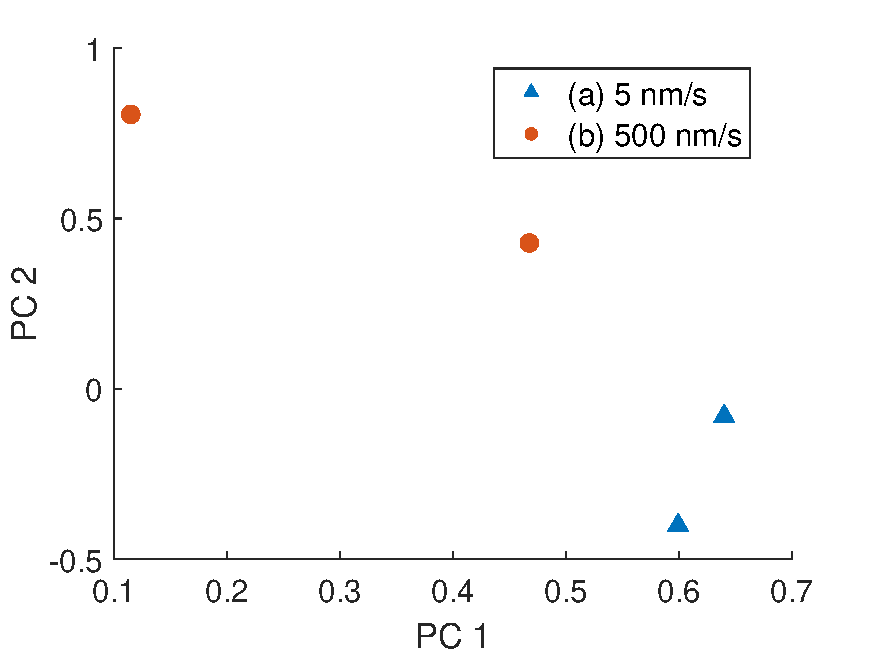
\includegraphics[width=\linewidth]{../data/Ni100_pca.pdf}
        \caption[First two principal components of the Ni strain-stress curves in $\langle 1\,0\,0 \rangle$.]{First two principal components of the Ni strain-stress curves in $\langle 1\,0\,0 \rangle$. First and second principal components respecitvely correspond to $79.41\%$ and $19.05\%$ of the observed variance between curves.}
        \label{sf:Ni100_pca}
    \end{subfigure}
    ~
    \begin{subfigure}[t]{0.45\linewidth}
        \centering
        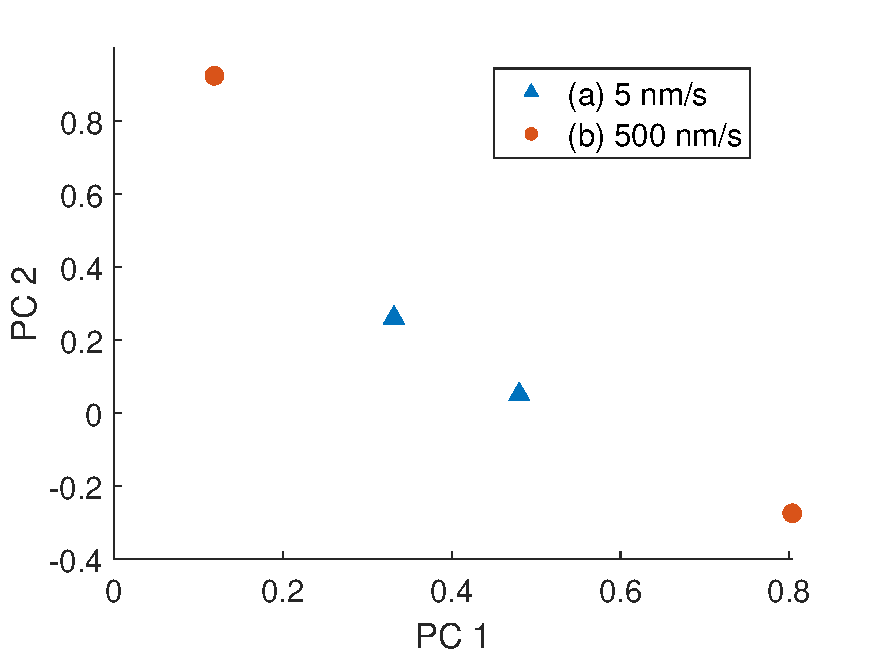
\includegraphics[width=\linewidth]{../data/Ni110_pca.pdf}
        \caption[First two principal components of the Ni strain-stress curves in $\langle 1\,1\,0 \rangle$.]{First two principal components of the Ni strain-stress curves in $\langle 1\,1\,0 \rangle$. First and second principal components respecitvely correspond to $70.61\%$ and $26.21\%$ of the observed variance between curves.}
        \label{sf:Ni110_pca}
    \end{subfigure}
    \caption{Blue triangles (\textcolor{matlabBlue}{$\blacktriangle$}) correspond to the $\SI{5}{\nano\metre\per\second}$ strain rate, orange circles (\textcolor{matlabOrange}{$\bullet$}) that of $\SI{500}{\nano\metre\per\second}$.}
    \label{f:Ni_pca}
\end{figure}

PCA also requires equivalent data, meaning readings must be taken with the same independent variables. In this case, the independent variable is strain while the dependent variable is stress. If there are no equivalent readings, inter- or extrapolation can be used. Extrapolation is unviable to compare the experimental to simulated curves as the difference in strain is too great. There was no need to interpolate experimental curves as the readings were all taken at equivalent strains. Doing PCA on the simulated curves would not provide additional insight, as the curves are very clearly different between large and small sources, as well as between different loading directions. Additionally, the plots comparing numeric and analytic tractions are quite clearly very similar. Lastly, there are very few samples, which is not enough for any form of clustering analysis. However, PCA could prove a useful tool in future works as comptutational capability and data availability increase.

In the $\langle 1\, 0\, 0 \rangle$ loading direction, the low strain rate measurements cluster together, hinting at similar behaviour. Moreover, the higher strain rates have a larger spread. The Eucledian distance from one of them is even smaller to both low strain rate measurements, than it is to its high strain rate counterpart. More measurements are needed to draw conclusions as to why this is the case. Regardless, it is relatively safe to assume the strain rate has a noticeable effect when loading the $\langle 1\, 0\, 0 \rangle$ direction for these specific rates. Such information is relevant for our simulations, as their strain rates were much higher than these, so we must expect the simulated curves to behave accordingly, and our conclusions must be extrapolated with this in mind.

The story is very different for the $\langle 1\, 1\, 0 \rangle$ loading direction. All graphs in \cref{sf:Ni110} look quite similar. They are markedly different to those in \cref{sf:Ni100}, but among themselves there do not seem to be large differences between low strain rate curves, (a) and (b), and high strain rate ones, (c) and (d). Having said that, curves (c) and (d) consistently experience higher stresses than (a) and (b). With so few samples, it is hard to say whether there is a notable difference.

\Cref{sf:Ni110_pca} confirms this, the Eucledian distance between both low strain rate curves (\textcolor{matlabBlue}{$\blacktriangle$}) is much smaller to one another than that between both high strain rate curves (\textcolor{matlabOrange}{$\bullet$}). With only two data points for each measurement, it is very difficult to assert whether there is a relationship between the first and second principal components that can be used to correlate a curve to its strain rate. We therefore cannot draw satisfacotry conclusions whether such differences in strain rate have much of an effect. Conventional wisdom is that it will, but we cannot quantify how much, so we must tread with care.

Qualitatively and quantitatively, the simulations do a good job at reproducing the experimental strain-stress curves. Comparing the yield points and features of \cref{sf:Ni100,sf:Ni110} with those of \cref{sf:Ni100_DDD,sf:Ni110_DDD} shows remarkable agreement between them. While the simulations cannot reach the same strains as the experiments, they appear to fall within experimental variation, excepting curve (a) of \cref{sf:Ni110_DDD}.

\begin{figure}
    \centering
    \begin{subfigure}[t]{0.45\linewidth}
        \centering
        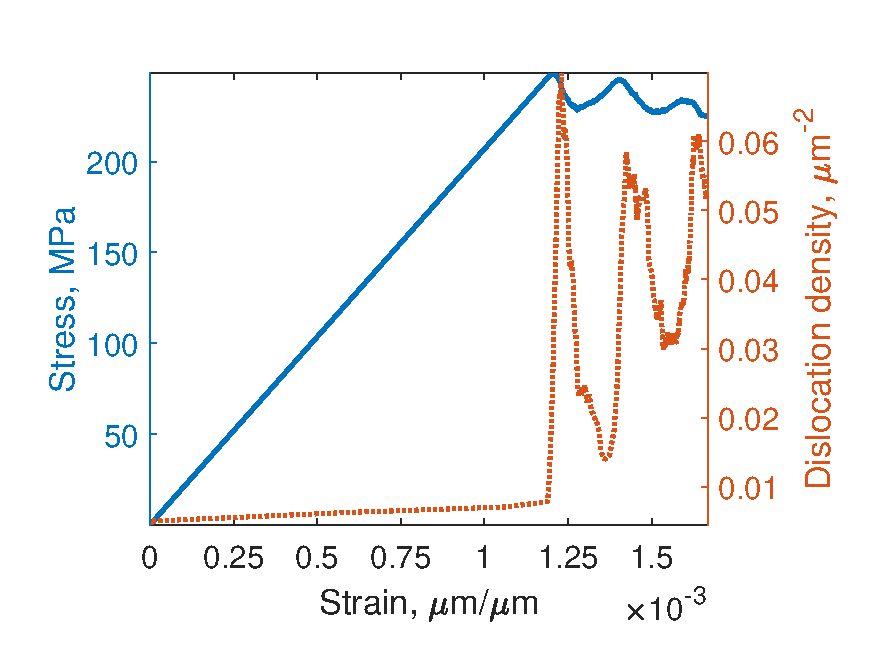
\includegraphics[width=\linewidth]{../data/density_11-Mar-2021_8_tensile_ni_100.pdf}
        \caption{$\langle 1\, 0\, 0 \rangle$, $L = \SI{0.8545}{\micro\metre}$, analytic tractions.}
        \label{sf:stressDens1}
    \end{subfigure}
    ~
    \begin{subfigure}[t]{0.45\linewidth}
        \centering
        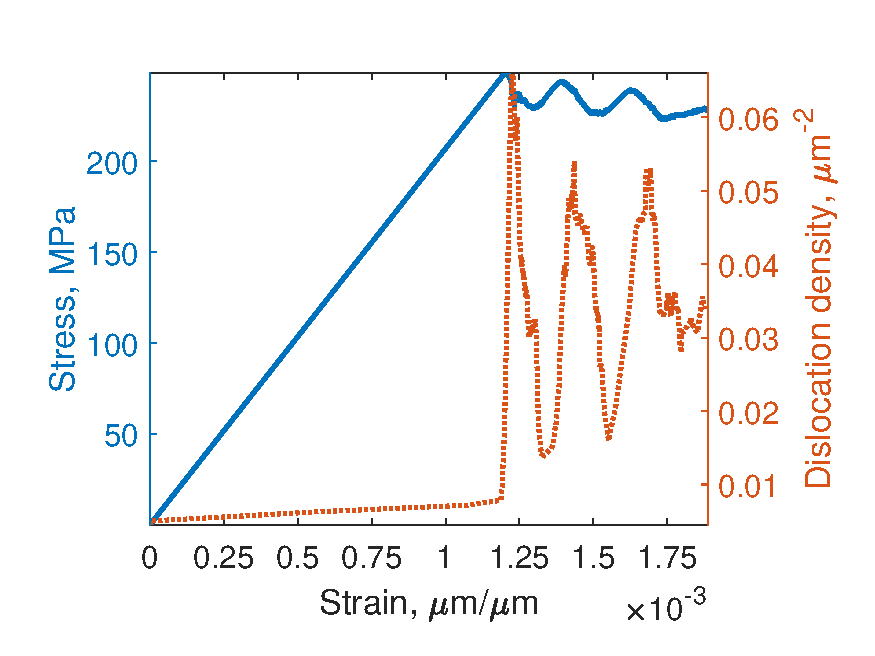
\includegraphics[width=\linewidth]{../data/density_11-Mar-2021_numT_8_tensile_ni_100.pdf}
        \caption{$\langle 1\, 0\, 0 \rangle$, $L = \SI{0.8545}{\micro\metre}$, numeric tractions.}
        \label{sf:stressDens2}
    \end{subfigure}

    \begin{subfigure}[t]{0.45\linewidth}
        \centering
        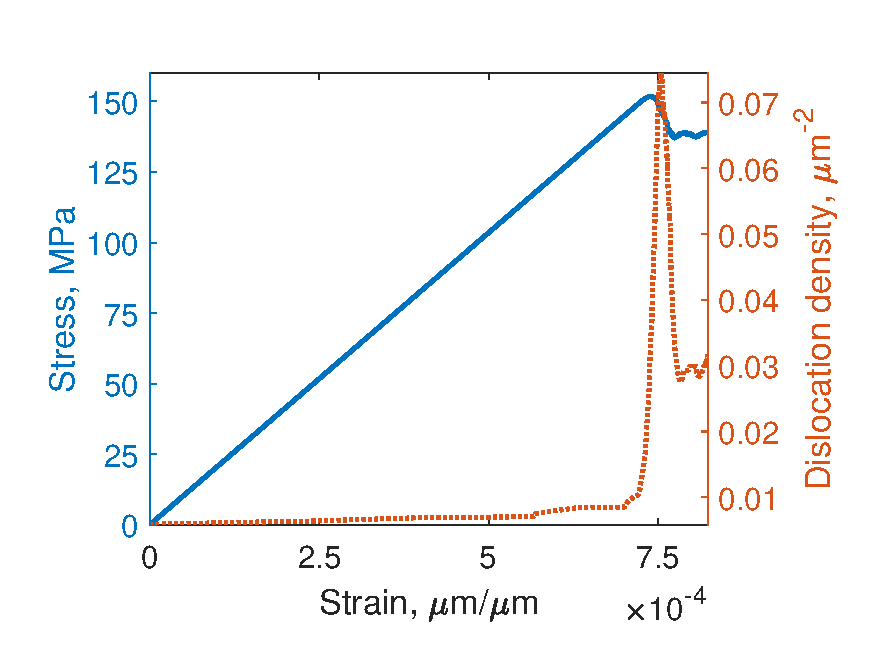
\includegraphics[width=\linewidth]{../data/density_16-Mar-2021_8_tensile_ni_100.pdf}
        \caption{$\langle 1\, 0\, 0 \rangle$, $L = \SI{1.1012}{\micro\metre}$, analytic tractions.}
        \label{sf:stressDens3}
    \end{subfigure}

    \begin{subfigure}[t]{0.45\linewidth}
        \centering
        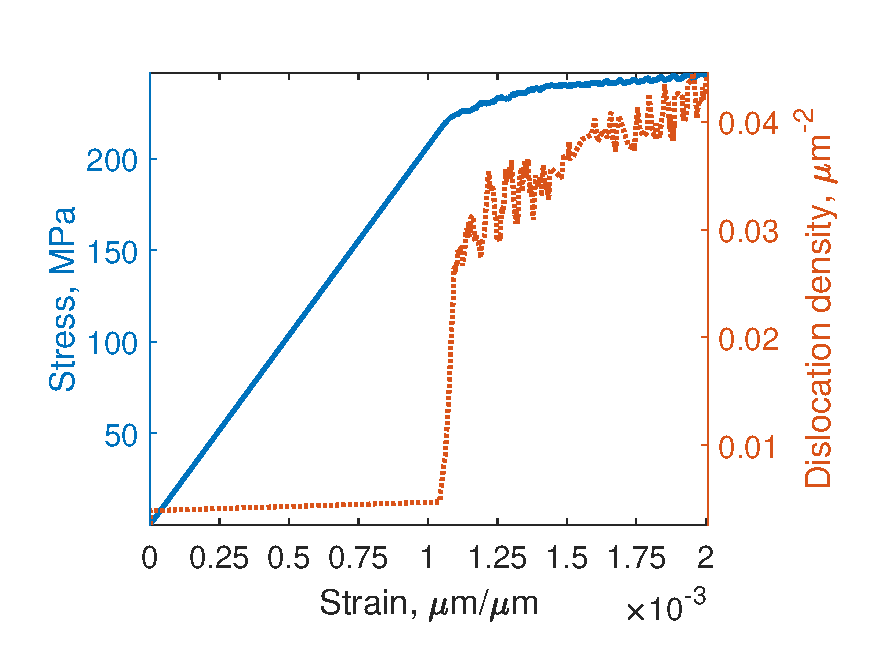
\includegraphics[width=\linewidth]{../data/density_11-Mar-2021_4_tensile_ni_110.pdf}
        \caption{$\langle 1\, 1\, 0 \rangle$, $L = \SI{0.9897}{\micro\metre}$, analytic tractions.}
        \label{sf:stressDens4}
    \end{subfigure}
    ~
    \begin{subfigure}[t]{0.45\linewidth}
        \centering
        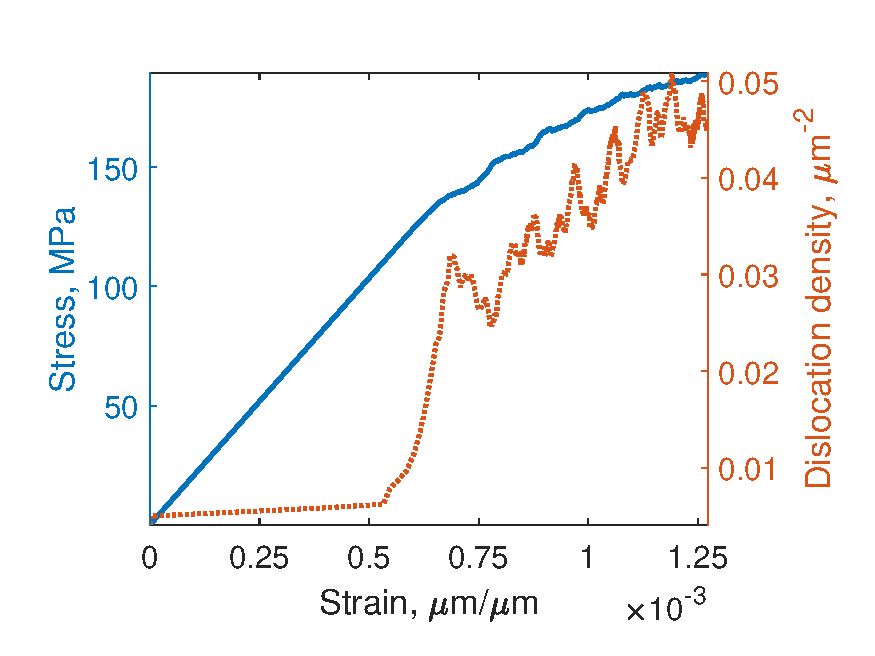
\includegraphics[width=\linewidth]{../data/density_16-Mar-2021_4_tensile_ni_110.pdf}
        \caption{$\langle 1\, 1\, 0 \rangle$, $L = \SI{1.5482}{\micro\metre}$, analytic tractions.}
        \label{sf:stressDens5}
    \end{subfigure}
    \caption{Strain-stress curves (blue solid lines) and dislocation densiti (orange dotted lines) for all 5 simulations.}
    \label{f:stressDens}
\end{figure}

That said, we must be aware that the strain rate is 5 million times higher than $\SI{5}{\nano\meter\per\second}$. As previously mentioned, this strain rate was arrived at by finding the highest one that would not exponentially increase the yield point. However, this does not mean lower strain rates do not decrease the yield point, they do, just not very drastically. They are also impractically slow for our needs. \Cref{f:strainRate} shows the effect of different strain rates on the same simulation.

\begin{figure}
    \centering
    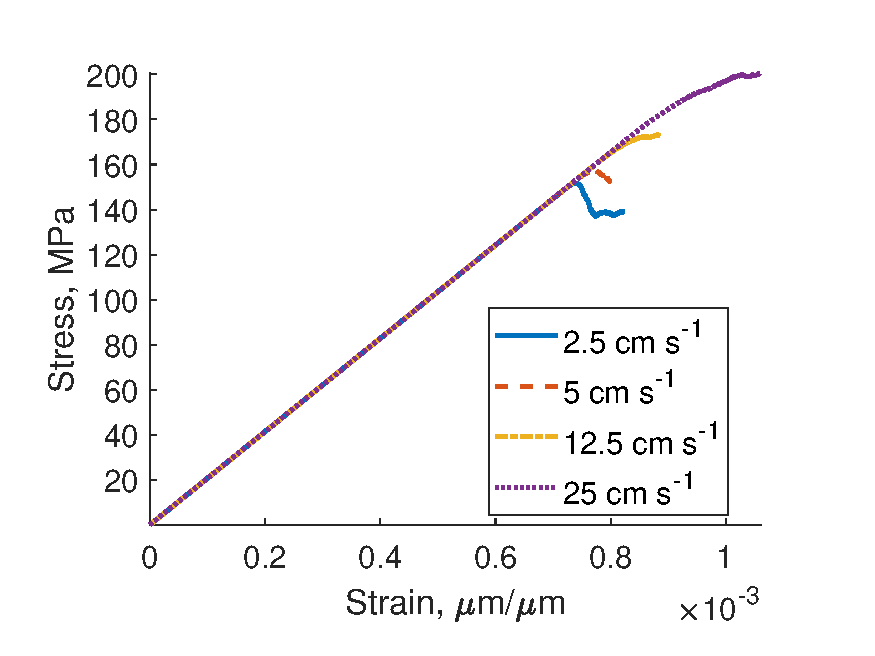
\includegraphics[width=0.8\linewidth]{../data/strainRate_16-Mar-2021_8_tensile_ni_100.pdf}
    \caption{Strain rate effect on the yield point of the same simulation in the $\langle 1\, 0\, 0 \rangle$ loding direction, $L = \SI{1.1012}{\micro\metre}$, using analytic tractions.}
    \label{f:strainRate}
\end{figure}

It is also interesting to note that this was achieved with very small dislocation densities (see \cref{t:sourceSize}), contrary to the originally assumed 10 dislocations \si{\micro\metre^{-2}}. They were also all prismatic and uniform in both size and shape. These are not wholly unreasonable assumptions, but they are definitely not strictly true, yet they did a remarkable job.

The appeal of dislocation plasticity is correlating dislocation dynamics to plastic behaviour. \Cref{f:stressDens} shows how the strain-stress curves are correlated to dislocation density. Stress is dissipated via dislocation motion, the more dislocation motion within a solid, the more stress is dissipated. Peaks and valleys in the strain-stress curve are correlated with peaks and valleys in the dislocation density. As the FR sources activate, the total internal dislocation length increases, increasing the dislocation density and so does the dislocation network's capacity to relax stresses. As dislocations exit the solid and create slip steps, the dislocation density and the network's capacity for relaxing stresses decrease. Once the FR sources pinch off, they can generate new loops and the process can start again. This cycle of increasing and decreasing dislocation density is a much more pronounced in the $\langle 1\, 0\, 0 \rangle$ loading direction (\cref{sf:stressDens1,sf:stressDens2,sf:stressDens3}) than in $\langle 1\, 1\, 0\rangle$ (\cref{sf:stressDens4,sf:stressDens5}), giving rise to the characteristic features of the strain-stress curves for each loading direction.

\Cref{c:tractions} showed that numeric tractions are numerically unstable. This can be seen when comparing the curve using analytic tractions (a) and the one using numeric ones (b) in \cref{sf:Ni100_DDD}.There is a jump at around $1.2\times 10^{-3}$ strain in (b). Furthermore, both curves start diverging from each other after $\sim 1.5\times 10^{-3}$. The reason can be seen in \cref{sf:stressDens1,sf:stressDens2} where the drops in dislocation density are much more drastic in the simulation that used numeric tractions. The dislocation density near $1.5\times 10^{-3}$ strain, in \cref{sf:stressDens2} is almost half of that in \cref{sf:stressDens1} as shown in \cref{sf:minDensAna,sf:minDensNum}. Once the density peaked again in \cref{sf:stressDens2} around $1.6\times 10^{-3}$ strain, it did not reach as high as its counterpart using analytic tractions in \cref{sf:stressDens1}. This gave the simulation using numeric tractions an edge over the more accurate one. This lower density also explains why the stresses diverged at higher values when using numeric tractions.

We cannot compare exactly equivalent points between simulations using numeric vs analytic tractions because the integrator is adaptive, but \cref{f:minMaxDens} shows the dislocation structures at the local dislocation density maximum and minimum between approximately $1.4$ to $1.6\times 10^{-3}$ strain, after which the simulations quickly diverged.

\begin{figure}
    \centering
    \begin{subfigure}[t]{0.45\linewidth}
        \centering
        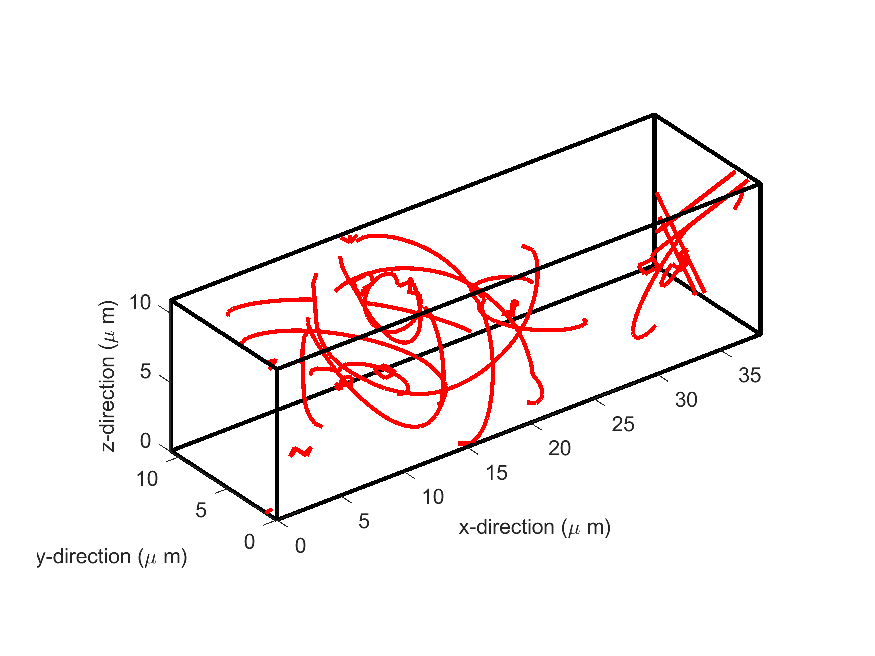
\includegraphics[width=\linewidth]{../data/maxDens_nSeg_547_nSegTot_4382_11-Mar-2021_8_tensile_ni_100.pdf}
        \caption[Structure at a local maximum dislocation density for the simulation using analytic tractions.]{Structure at a local maximum dislocation density for the simulation using analytic tractions. $\rho = 5.84 \times 10^{-2}$ dislocations \si{\micro\metre^{2}} at $ 1.43\times 10^{-3}$ strain, 547 internal segments and 4382 total segments.}
        \label{sf:maxDensAna}
    \end{subfigure}
    ~
    \begin{subfigure}[t]{0.45\linewidth}
        \centering
        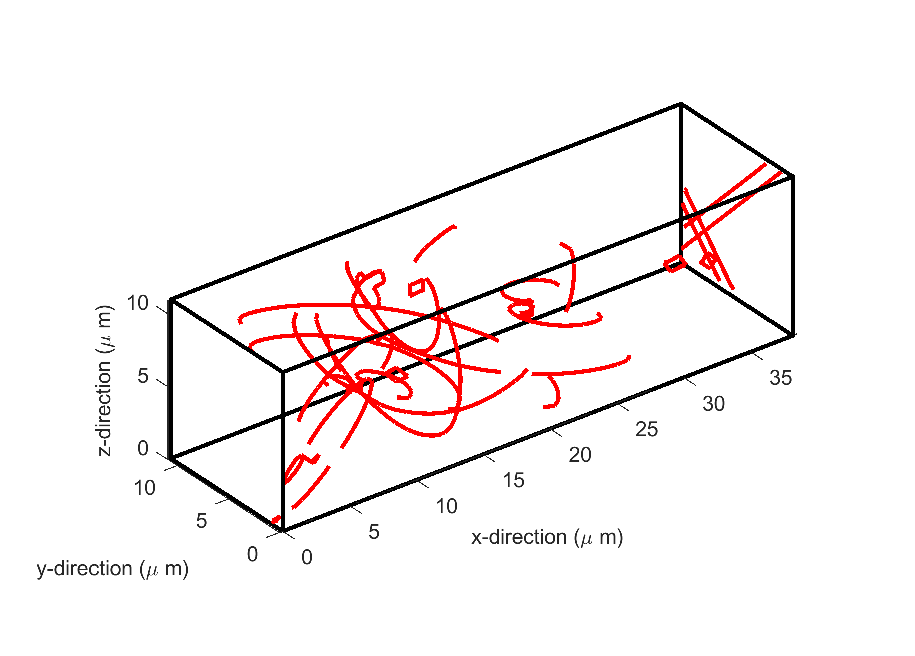
\includegraphics[width=\linewidth]{../data/maxDens_nSeg_529_nSegTot_4819_11-Mar-2021_numT_8_tensile_ni_100.pdf}
        \caption[Structure at a local maximum dislocation density for the simulation using analytic tractions.]{Structure at a local maximum dislocation density for the simulation using numeric tractions. $\rho = 5.41\times 10^{-2}$ dislocations \si{\micro\metre^{2}} at $1.44 \times 10^{-3}$ strain, 529 internal segments and 4819 total segments.}
        \label{sf:maxDensNum}
    \end{subfigure}

    \begin{subfigure}[t]{0.45\linewidth}
        \centering
        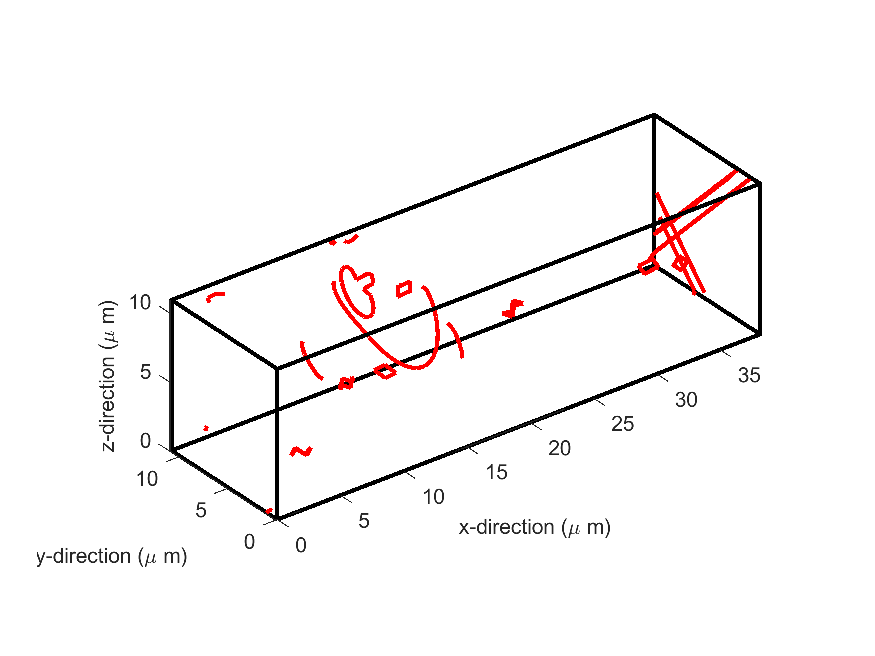
\includegraphics[width=\linewidth]{../data/minDens_nSeg_317_nSegTot_7179_11-Mar-2021_8_tensile_ni_100.pdf}
        \caption[Structure at a local minimum dislocation density for the simulation using analytic tractions.]{Structure at a local minimum dislocation density for the simulation using analytic tractions. $\rho = 2.99\times 10^{-2}$ dislocations \si{\micro\metre^{2}} at $1.54\times 10^{-3}$ strain, 317 internal segments and 7179 total segments.}
        \label{sf:minDensAna}
    \end{subfigure}
    ~
    \begin{subfigure}[t]{0.45\linewidth}
        \centering
        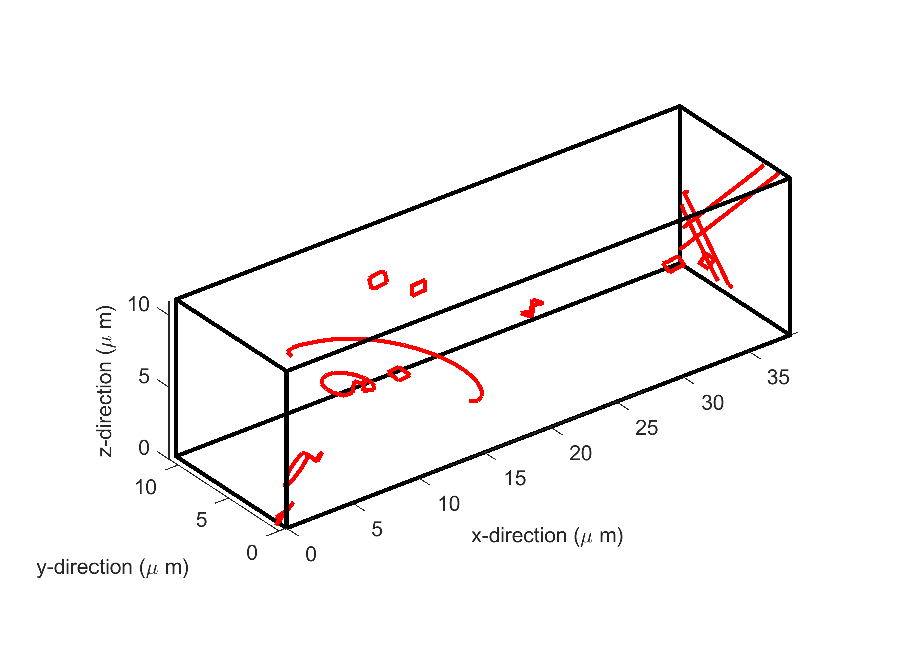
\includegraphics[width=\linewidth]{../data/minDens_nSeg_204_nSegTot_8204_11-Mar-2021_numT_8_tensile_ni_100.pdf}
        \caption[Structure at a local minimum dislocation density for the simulation using analytic tractions.]{Structure at a local minimum dislocation density for the simulation using numeric tractions. $\rho = 1.6\times 10^{-2}$ dislocations \si{\micro\metre^{2}} at $1.6 \times 10^{-3}$ strain, 204 internal segments and 8204 total segments.}
        \label{sf:minDensNum}
    \end{subfigure}
    \caption{Dislocation structures for simulations using analytic vs numeric tractions in the loading direction $\langle 1\, 0\, 0\rangle$, and source segment length $L = \SI{0.8545}{\micro\metre}$.}
    \label{f:minMaxDens}
\end{figure}

In this case, the numeric tractions managed to get further than the analytic ones, but this is not always true. If the network is sensitive to the instabilities of numeric tractions, simulations can be negatively impacted by the incorrect movement of segments (see \cref{f:simulation}). The reason numeric tractions got further in this case is quite simple. A universally observed feature of numeric tractions, is evidenced by the total number segments in \cref{f:minMaxDens}. The simulations using numeric tractions generated more segments at roughly equivalent points than their analytic counterparts. The number of extra segments grew as the simulations advanced, from an extra $10\%$ in \cref{sf:maxDensNum} with respect to \cref{sf:maxDensAna}, to an extra $14\%$ in \cref{sf:minDensNum} compared to \cref{sf:minDensAna}. However, not only were segments generated more readily, but they exited the domain more quickly, as evidenced by simultaneously having more total segments, but fewer internal ones, in both absolute and relative terms. As mentioned in \cref{c:topology}, external segments are only used to keep track of slip steps, so they are computationally much cheaper than internal ones. Simulations where segments cannot leave the domain so readily are slowed down by virtue of there being more internal segments. For example, cantilever bending has a neutral axis where segments pile up, and nanoindentation pushes segments into the simulation domain. We have also anecdotally observed in cantilever simulations, that dislocations pile up near the neutral axis much closer to one another when using numeric tractions as opposed to analytic ones, which is likely the result of faster moving segments (though a more formal investigation is needed to confirm this). Clearly, further study of other non-trivial emergent behaviours would help us provide better guidelines for different use cases of EasyDD. For the time being, as mentioned in \cref{c:topology,c:tractions}, we have found the analytic tractions to be much more robust and reliable, so the recommendation is to use them if available.

We have also produced \texttt{mp4} videos showing the evolution of the dislocation structure alongside the strain-stress curve for the simulations in \cref{f:NiStrainStress} found in \href{https://github.com/dcelisgarza/DPhil_Thesis/tree/master/data}{https://github.com/dcelisgarza/DPhil\_Thesis/tree/master/data}.

The final aspect of reproducing experimental results with dislocation plasticity is to see what the slip steps look like. Again, given the time scales and small strains we can simulate with dislocation plasticity, we will not see slip steps that are as large as those experimentally observed. Each exited dislocation with Burgers vector $\vec{b}$ will create a corresponding slip step with the same vector and magnitude. As more loops generated by the FR source keep exiting the domain, the slip step grows by $b$ each time one of them exits the surface. Using the dislocation-induced displacements described in \cite{bromage2018calculating}, we plot the slip steps at the final states of our simulations in \cref{f:slipSteps}.

\begin{figure}
    \centering
    \begin{subfigure}[t]{0.45\linewidth}
        \centering
        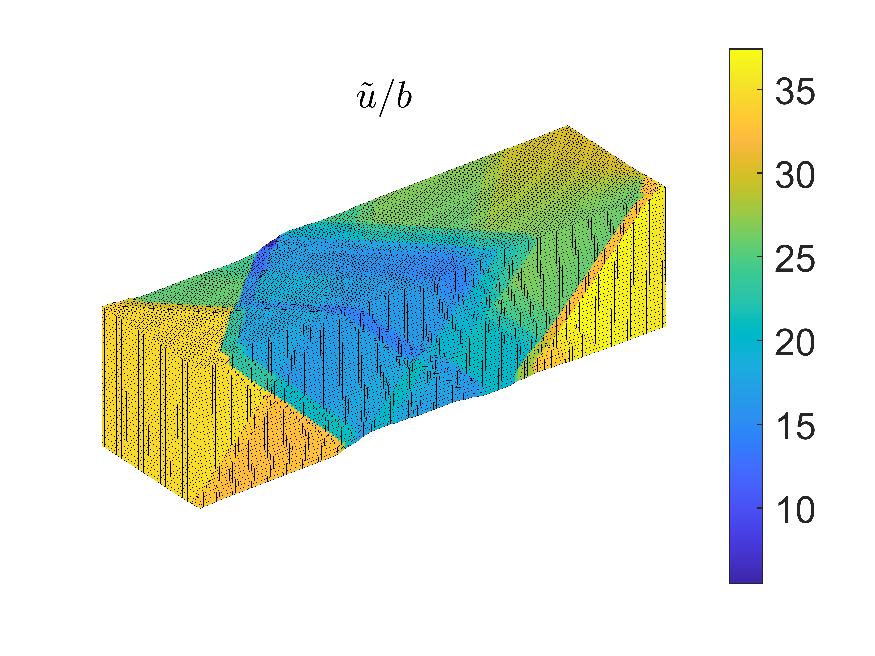
\includegraphics[width=\linewidth]{../data/11-Mar-2021_8_tensile_ni_100_196800_disp.pdf}
        \caption{Tensile loading in $\langle 1\, 0\, 0 \rangle$. Corresponds to (a) in \cref{sf:Ni100_DDD} (analytic tractions).}
        \label{sf:Ni100a_disp}
    \end{subfigure}
    ~
    \begin{subfigure}[t]{0.45\linewidth}
        \centering
        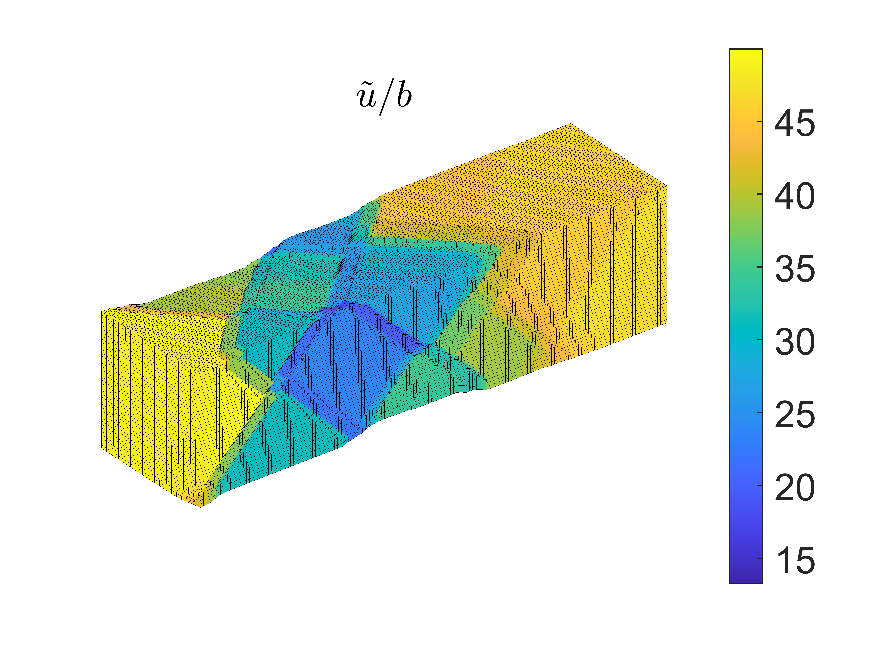
\includegraphics[width=\linewidth]{../data/11-Mar-2021_numT_8_tensile_ni_100_168600_disp.pdf}
        \caption{Tensile loading in $\langle 1\, 0\, 0 \rangle$. Corresponds to (b) in \cref{sf:Ni100_DDD} (numeric tractions).}
        \label{sf:Ni100aN_disp}
    \end{subfigure}

    \begin{subfigure}[t]{0.45\linewidth}
        \centering
        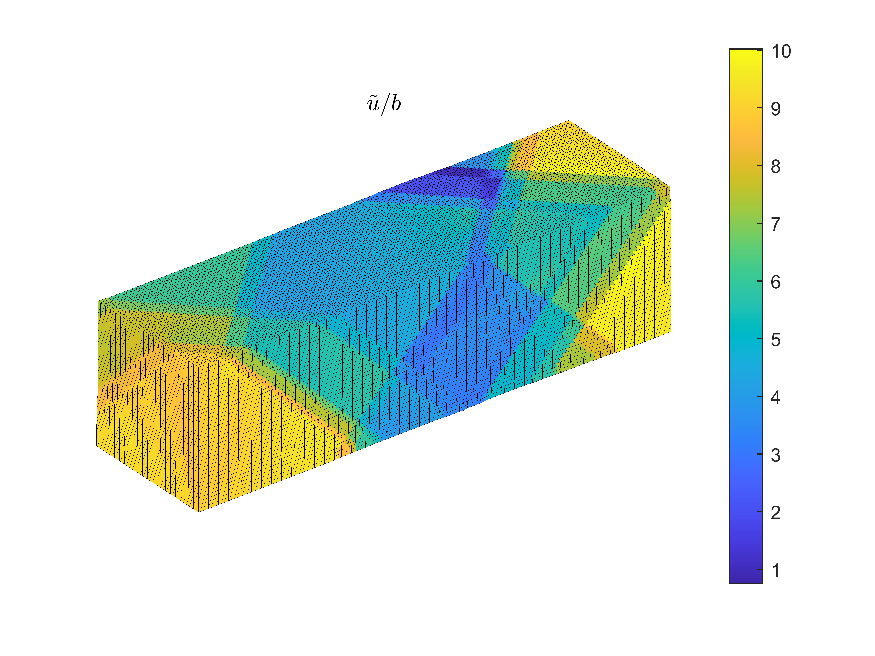
\includegraphics[width=\linewidth]{../data/16-Mar-2021_8_tensile_ni_100_214400_disp.pdf}
        \caption{Tensile loading in $\langle 1\, 0\, 0 \rangle$. Corresponds to (c) in \cref{sf:Ni100_DDD}.}
        \label{sf:Ni100b_disp}
    \end{subfigure}

    \begin{subfigure}[t]{0.45\linewidth}
        \centering
        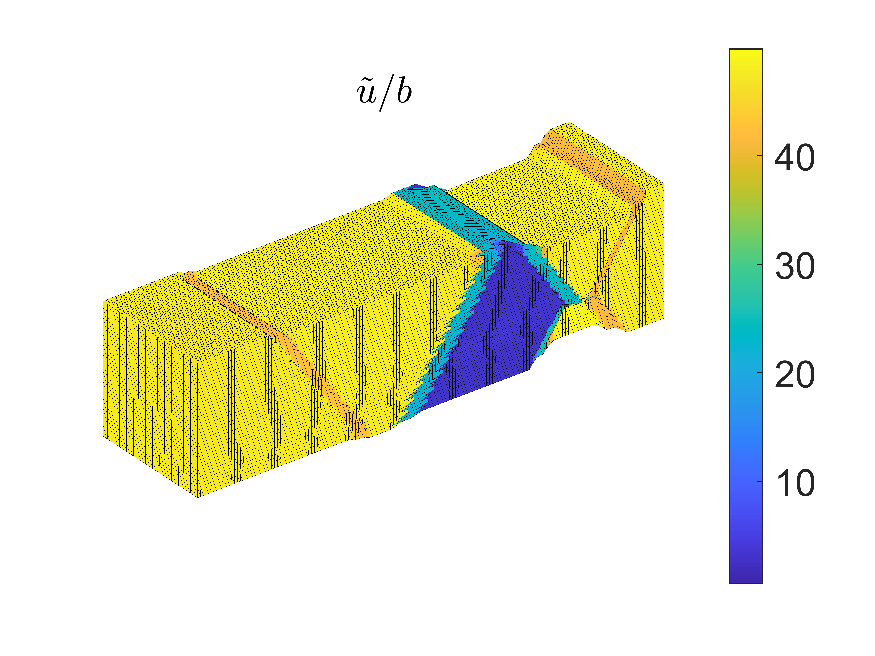
\includegraphics[width=\linewidth]{../data/11-Mar-2021_4_tensile_ni_110_205600_disp.pdf}
        \caption{Tensile loading in $\langle 1\, 1\, 0 \rangle$. Corresponds to (a) in \cref{sf:Ni110_DDD}.}
        \label{sf:Ni110a_disp}
    \end{subfigure}
    ~
    \begin{subfigure}[t]{0.45\linewidth}
        \centering
        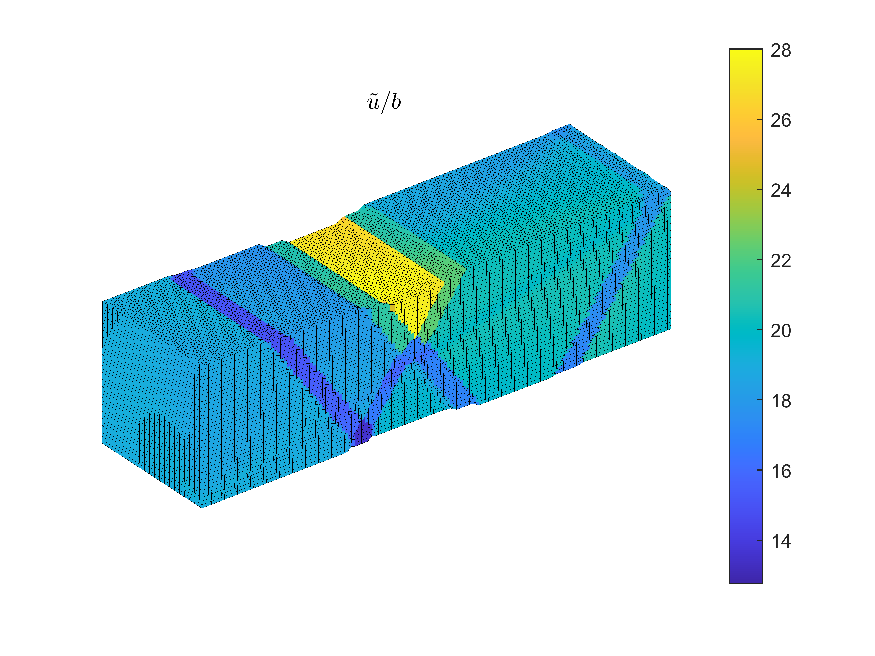
\includegraphics[width=\linewidth]{../data/16-Mar-2021_4_tensile_ni_110_225000_disp.pdf}
        \caption{Tensile loading in $\langle 1\, 1\, 0 \rangle$. Corresponds to (b) in \cref{sf:Ni110_DDD}.}
        \label{sf:Ni110b_disp}
    \end{subfigure}
    \caption[Slip steps normalised to Burgers vector magnitude for the final states of tensile loading simulations.]{Slip steps normalised to Burgers vector magnitude for the final states of tensile loading simulations. The displacements are scaled $100\times$ for display purposes, the colour bars are not scaled.}
    \label{f:slipSteps}
\end{figure}

The first thing of note is the fact that the slip steps of simulations with higher strain present larger slip steps than other simulations of the same system. The second thing is that for the $\langle 1\, 0\, 0 \rangle$ loading direction, the numeric tractions (\cref{sf:Ni100aN_disp}) produce one slip step that is much larger than the corresponding one in (\cref{sf:Ni100a_disp}). This is not an artifact of the fact that the numeric tractions achieved a larger strain. In reality, it is due to the increased activity of the source closest to the origin compared to the analytic counterpart. This is readily observed in the aformentioned videos.

Unfortunately we do not have experimental imaging data corresponding to the $\langle 1\, 1\, 0 \rangle$ loading direction, but the slip step patterns of \cref{sf:Ni100a_disp,sf:Ni100aN_disp,sf:Ni100b_disp} are \emph{very} similar to those observed in \cref{f:Ni100_disp}, including the criss-crossing of slip steps. Granted, the slip steps from the simulations are not remotely of the same magnitude; nor are they in the same places; and likely not with the same distribution as it appears the real dislocations are mostly located near the ends of the pillar, where it starts curving into the bulk; but they are extremely similar. That said, in all plots of \cref{f:slipSteps}, except \cref{sf:Ni110b_disp}, the largest slip steps are also concentrated near the ends of the simulation domain. One could even argue \cref{f:slipSteps} shows the beginning of necking, as observed in \cref{sf:necking}.
\begin{figure}
    \centering
    \begin{subfigure}[t]{0.45\linewidth}
        \centering
        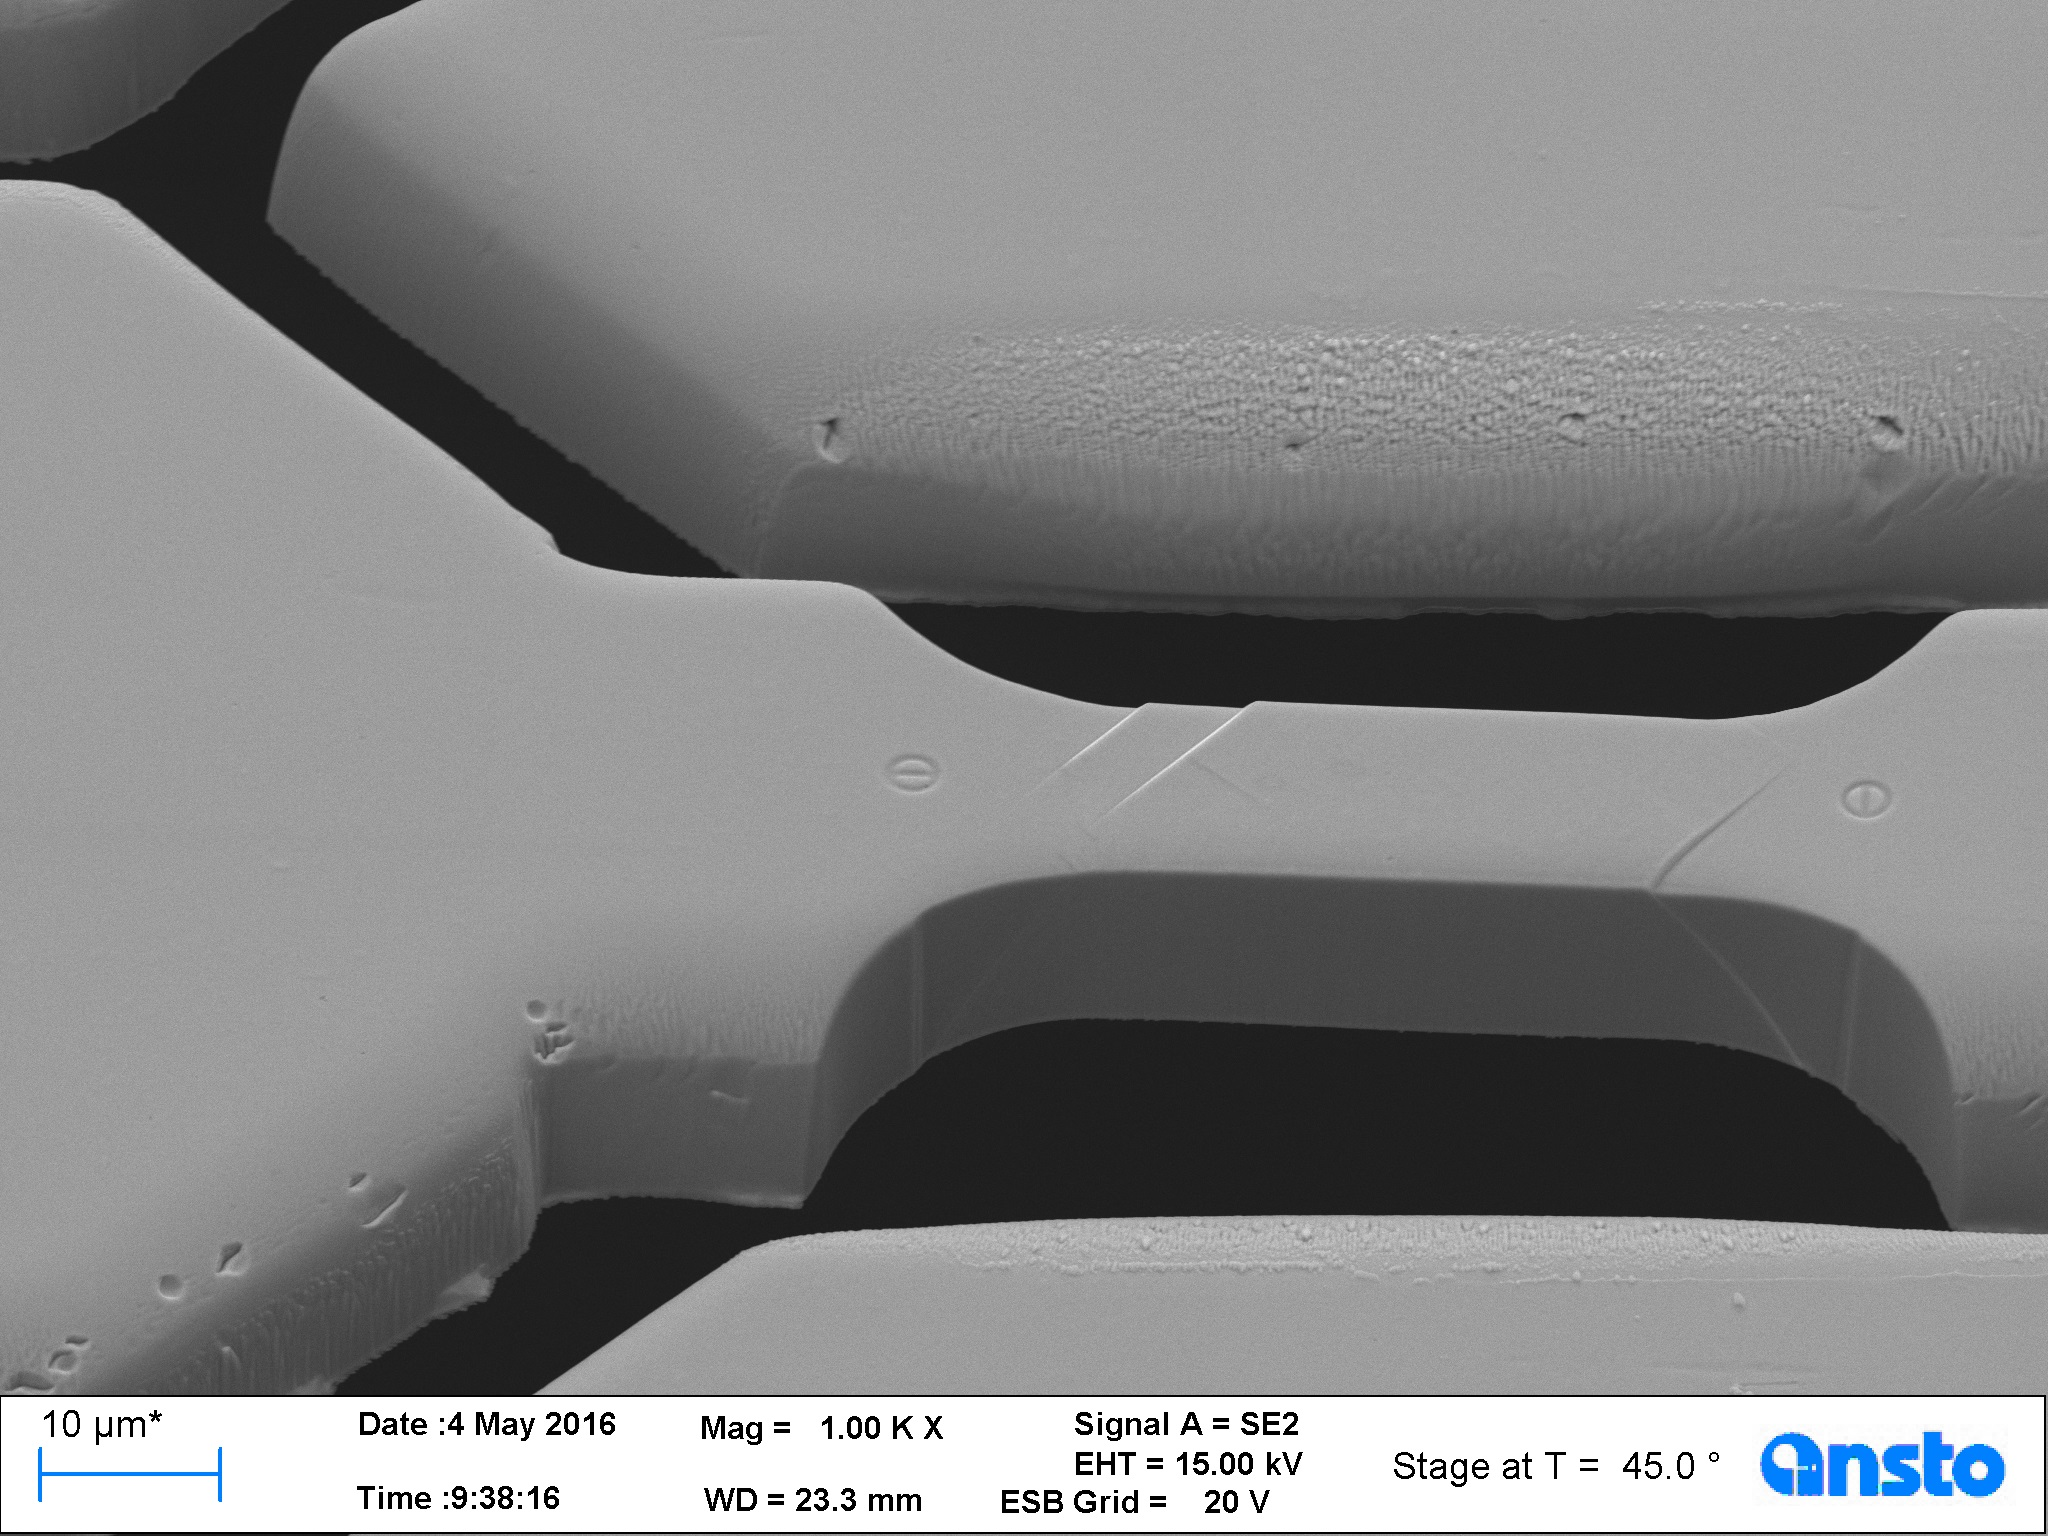
\includegraphics[width=\linewidth]{../data/Ni016.jpg}
        \caption{}
    \end{subfigure}
    ~
    \begin{subfigure}[t]{0.45\linewidth}
        \centering
        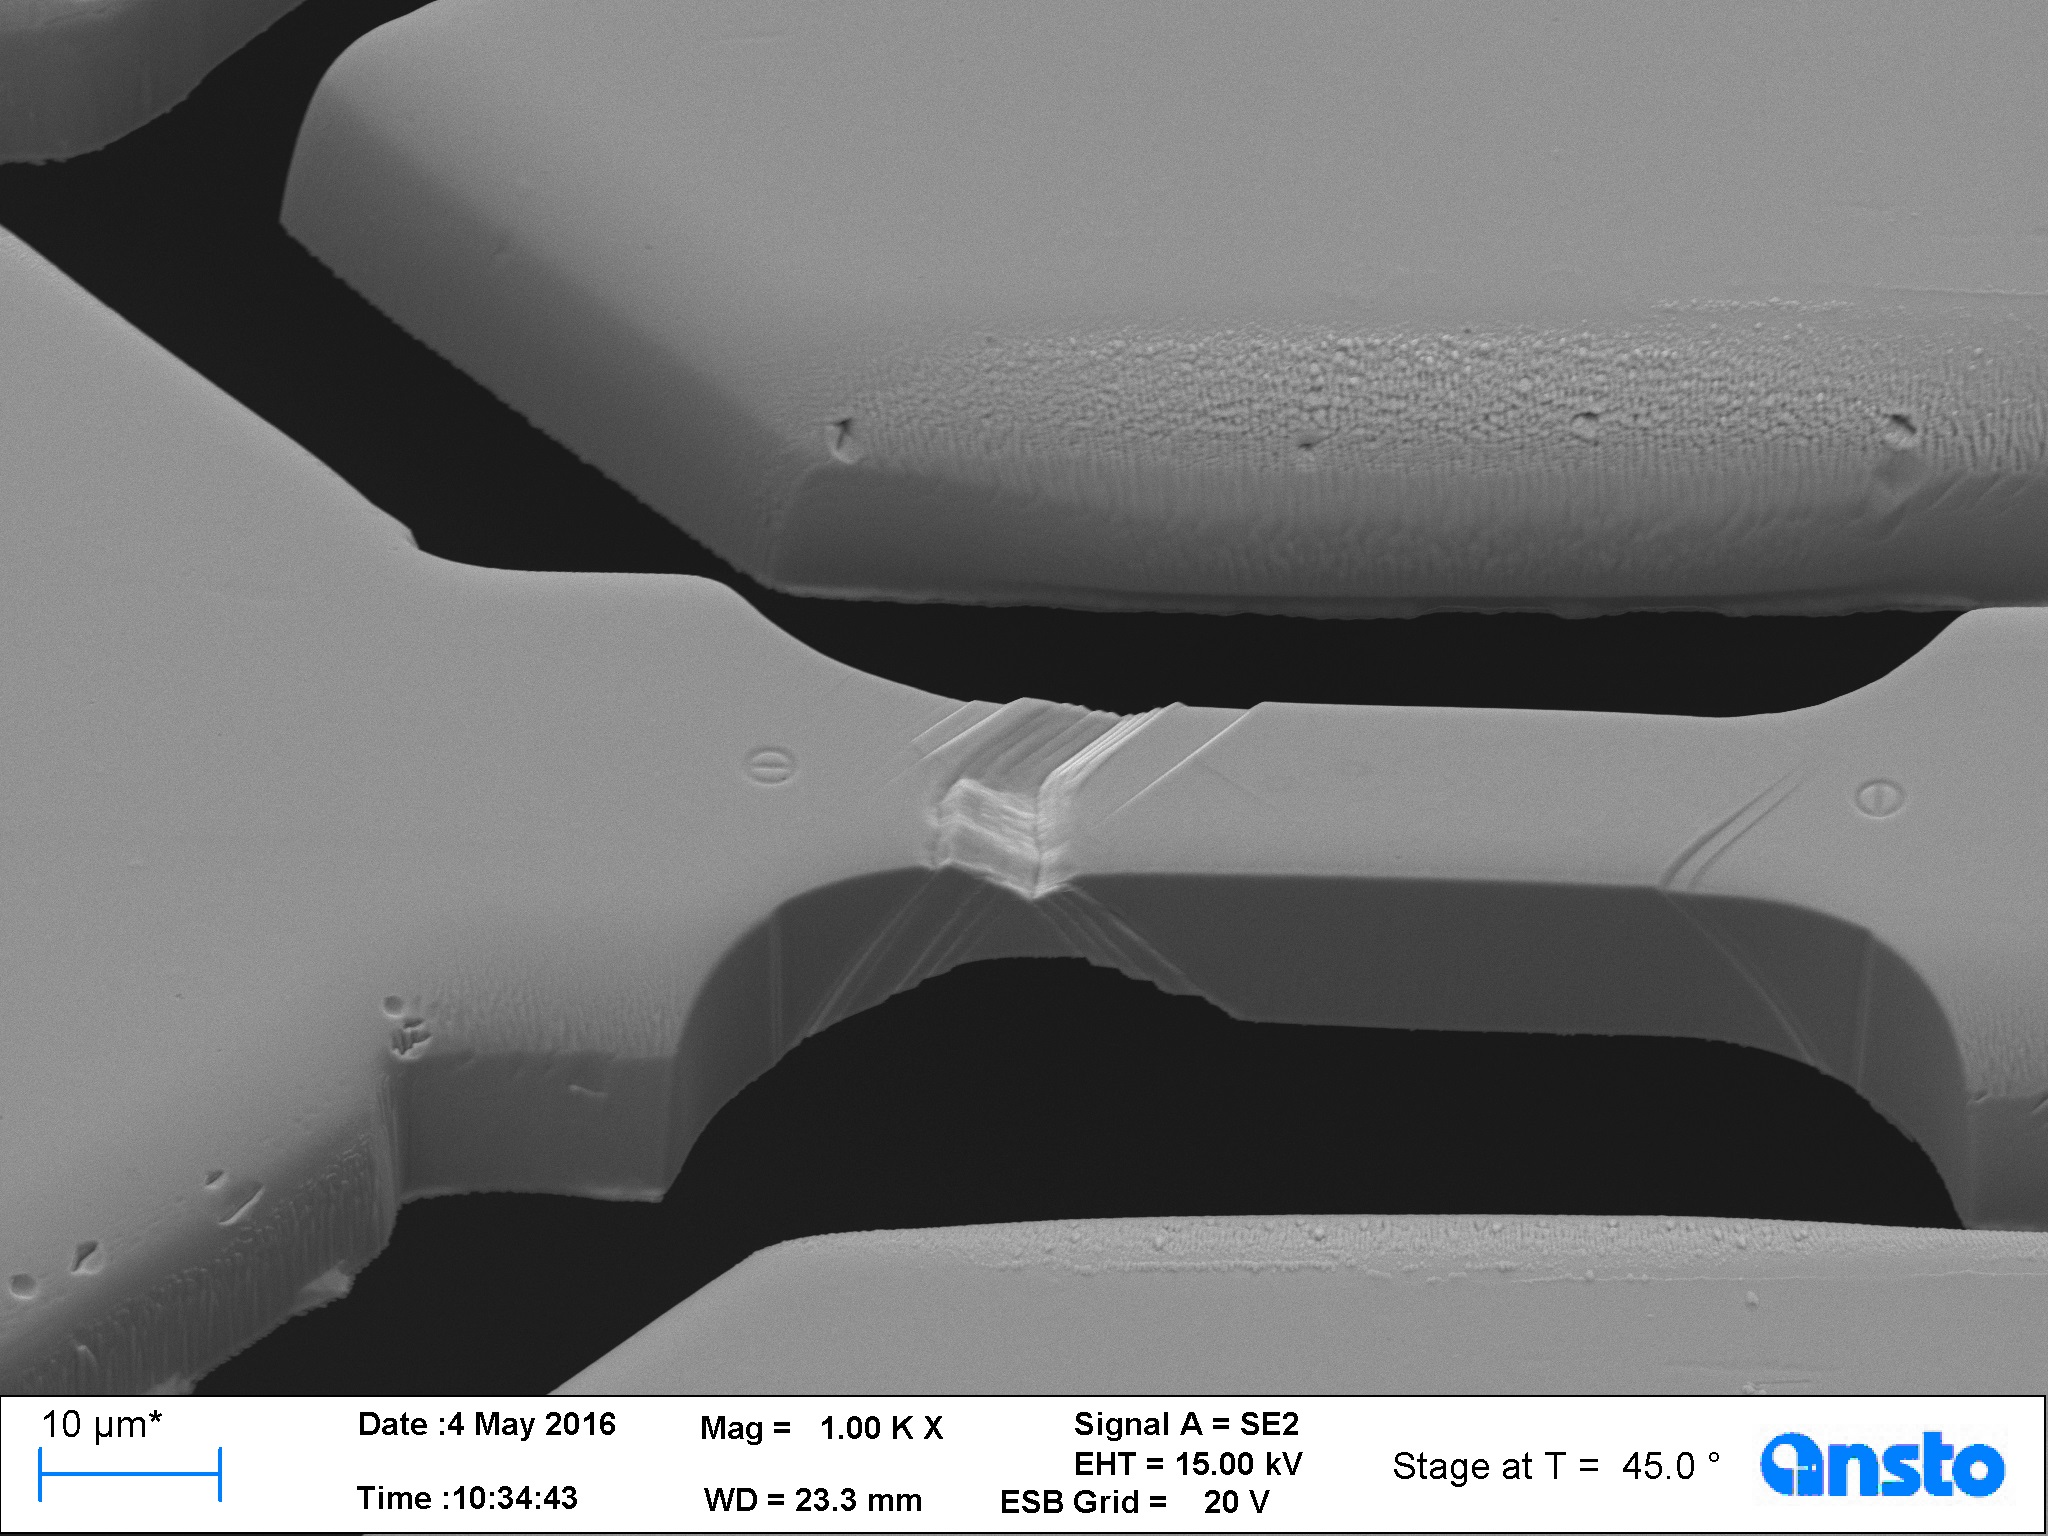
\includegraphics[width=\linewidth]{../data/Ni023.jpg}
        \caption{}
        \label{sf:necking}
    \end{subfigure}
    \caption[SEM images of tensile test in $\langle 1\, 0\, 0 \rangle$.]{SEM images of tensile test in $\langle 1\, 0\, 0 \rangle$. (a) shows slip steps forming. (b) shows necking as the strain increases. Provided courtesy of Alan Xu and Dhriti Bhattacharyya from ANSTO Sydney.}
    \label{f:Ni100_disp}
\end{figure}

\Cref{f:Ni100_disp} shows a few slip steps (and eventual necking) near the ends of the micropillar. These steps are at $45 \deg$ with respect to the square cross-section. The camera is also $45 \deg$ with respect to the top surface with normal, $\vec{n}_\rvar{surf} = [0\, 0\, 1]$. However, the camera is not perfectly perpendicular to the $\langle 1\, 0\, 0 \rangle$ direction and the focusing makes exactly following the slip steps difficult, so the measured angle with ImageJ \cite{imagej} is not exactly $45 \cos(\pi/4) \deg \approx 31.82 \deg$, but between $40$ and $35 \deg$ depnding on how the measurements are taken. The line traced by the slip steps is given by $\vec{l} \coloneqq \vec{n}_\rvar{slip} \times \vec{n}_\rvar{surf}$, where $\vec{n}_\rvar{slip}$ is the dislocation's slip plane normal. Here $\vec{l} = [1\, 1\, 0]$, so $\vec{n}_\rvar{slip} = \left(\overline{1}\, 1\, 1\right)$, which is found in \cref{t:slipSystems} and whose $\vec{b} = [1\, 0\, 1]$. The leftmost side of \cref{sf:Ni100a_disp,sf:Ni100aN_disp,sf:Ni100b_disp} clearly show this exact slip step.

With the resolution of the SEM images, it is hard to tell exactly how many slip steps there are in the experimental measurements. Furthermore, the simulations have not reached anywhere near the strains of the experiments. However, it is clearly evident that we can reproduce the phenomenology behind experimental observations in very fine detail thanks to dislocation plasticity, at least at small strains.

\section{Conclusions}
\label{s:concSim}

The point of dislocation plasticity simulations is to provide insight as to the mechanisms behind plasticity. Even with its limitations to small strains, its strong assumptions, and the necessity for extremely high strain rates, it can offer insight and explain the phenomena we can experimentally observe.

We made some very strong assumptions in \cref{ss:modelSetup} regarding the distribution, size, number and participating slip systems. Obtaining these parameters for things such as micropillars is impossible, one may be able to use a TEM sample as a proxy and make an educated guess from there. However, we have shown that some very simple assumptions with very few sources work remarkably well, at least when the sample is monocrystalline as was the case here. It is hard to extrapolate whether such simple assumptions with so few sources are appropriate for other types of simulations, but there may be some wisdom that can be gleaned from this. Perhaps it is better and more accurate to increase the size of the sources rather than their number, as well as dropping the strain rates as low as practically viable.

We managed to show slip steps and the beginning of necking behaviour that closely follow experimental patterns. We also managed to reproduce the yield stresses for both $\langle 1\, 0\, 0 \rangle$ and $\langle 1\, 1\, 0 \rangle$ loading directions, to within experimental variation even when using much larger strain rates. The $\langle 1\, 0\, 0 \rangle$ simulations also showed the ``bumpiness'' of the experimental data, the reasons behind it, as well as how and why it differs from what is observed when loading the $\langle 1\, 1\, 0 \rangle$ direction.

Unfortunately, the spatial and time scales of dislocation plasticity, as well as the practical constraints of time and computational resources did not allow us to reach the same strains as the experiments. So we cannot be sure how the curves will behave going forward. Doubtless the stresses would increase, but would we see the dramatic increases and dips in stresses as the strains increase? The experimental setup is not sensitive enough to probe such small strains, so the simulations can only serve as a bridge between atomic and microscopic scales.

We also only included active slip systems in either loading direction, so the question remains as to how including the inactive systems would affect the results. Our results point towards this assumption being sound, but a future avenue of research would be to include them in future simulations.

The results presented in this chapter are the culmination of meeting the objectives posed for this DPhil, as stated in \cref{s:objectives}. It makes use of the work described in all the other chapters (except for the power dissipation criteria for collision-serparation) and barely scratches at the surface of the remarkable capabilities of dislocation plasticity and EasyDD.
\savearabiccounter
% 4090

